\documentclass[xcolor={dvipsnames}]{beamer}

\usetheme{Malmoe}
\usecolortheme{seagull}
\usepackage[]{natbib}
\usepackage{textpos}
\usepackage{amsmath, amssymb, bm}
\usepackage{multirow}
\usepackage{framed}
\usepackage{schemata}
\setbeamertemplate{navigation symbols}{}
\usepackage[english]{babel}
\usepackage{animate}
\usepackage{graphics}
\usepackage{fontawesome}


\definecolor{lightblue}{rgb}{0.145,0.6666,1} % Defines the color used for content box headers
\definecolor{Red}{rgb}{0.9,0.15,0}
\definecolor{Blue}{RGB}{55,126,184}
\definecolor{Green}{RGB}{77,175,74}
\definecolor{White}{RGB}{255,255,255}
\definecolor{Lightgray}{rgb}{0.86,0.86,0.86}

\setbeamertemplate{footline}
{
	\leavevmode%
	\hbox{%
		\begin{beamercolorbox}[wd=.50\paperwidth,ht=2.25ex,dp=1ex,center]{author in head/foot}%
			\usebeamerfont{author in head/foot}\insertshortauthor%% \beamer@ifempty{\insertshortinstitute}{}{(\insertshortinstitute)}
		\end{beamercolorbox}%
%		\hskip2pt%
		\begin{beamercolorbox}[wd=.50\paperwidth,ht=2.25ex,dp=1ex,center]{title in head/foot}%
			\usebeamerfont{title in head/foot}\insertshorttitle~~~~~~~~~~~~~~~~~~~~~~~~~~\insertframenumber
		\end{beamercolorbox}%
	}%
	\vskip0pt%
}
\makeatother

\title[Mexico's epidemic of violence]{}

\subtitle{\Large{\textsc{Mexico's upsurge of violence and its impact on life expectancy and lifespan inequality}}\\$\,$\\}


\author[JM Aburto. CPop meeting]
{
	\vspace{-0.5cm}
	\texorpdfstring{
		\begin{columns}
			\column{.9\linewidth}
			\centering
			\Large{Jos\'{e} Manuel Aburto}\\
			$\,$\\
			
\includegraphics[scale=0.2]{Figures/SDU_Logo.jpg}\\     
				\vspace{0.5cm}
%						\includegraphics[scale=0.2]{Figures/MPIDR.PNG}     
		\end{columns}
	}
	{}
}

\date[]{ November 2018}

\beamertemplatenavigationsymbolsempty
\begin{document}


\begin{frame}[plain]
	\titlepage
\end{frame}
%%%%%%%%%%%%%%%%%%%%%%%%%%%%%%%%%%%%%%%%%%%%%%%%%%%%%%%%%%%%%%%%%%%%%%%%%
%%%%%%%%%%%%%%%%%%%%%%%%%%%%%%%%%%%%%%%%%%%%%%%%%%%%%%%%%%%%%%%%%%%%%%%%%


%%%%%%%%%%%%%%%%%%%%%%%%%%%%%%%%%%%%%%%%%%%%%%%%%%%%%%%%%%%%%%%%%%%%%%%%%
\begin{frame}
	\LARGE{
		\begin{itemize}
		
			\item<1-> \textbf{Latin America} is the world's most \textbf{violent} region.
		
			\item<2-> This region has the \textbf{highest} homicide rate in the world (16.3 per 100,000).
		
    	    \item<3-> Central American countries $\longrightarrow$ \textbf{upsurge} of violence in the new century.
		
		\end{itemize}
		
	}

\end{frame}


\begin{frame}
	\begin{center}
		\Large{In Mexico: homicides declined in 2000-2005}
	\end{center}

	\hspace*{-1cm}   
	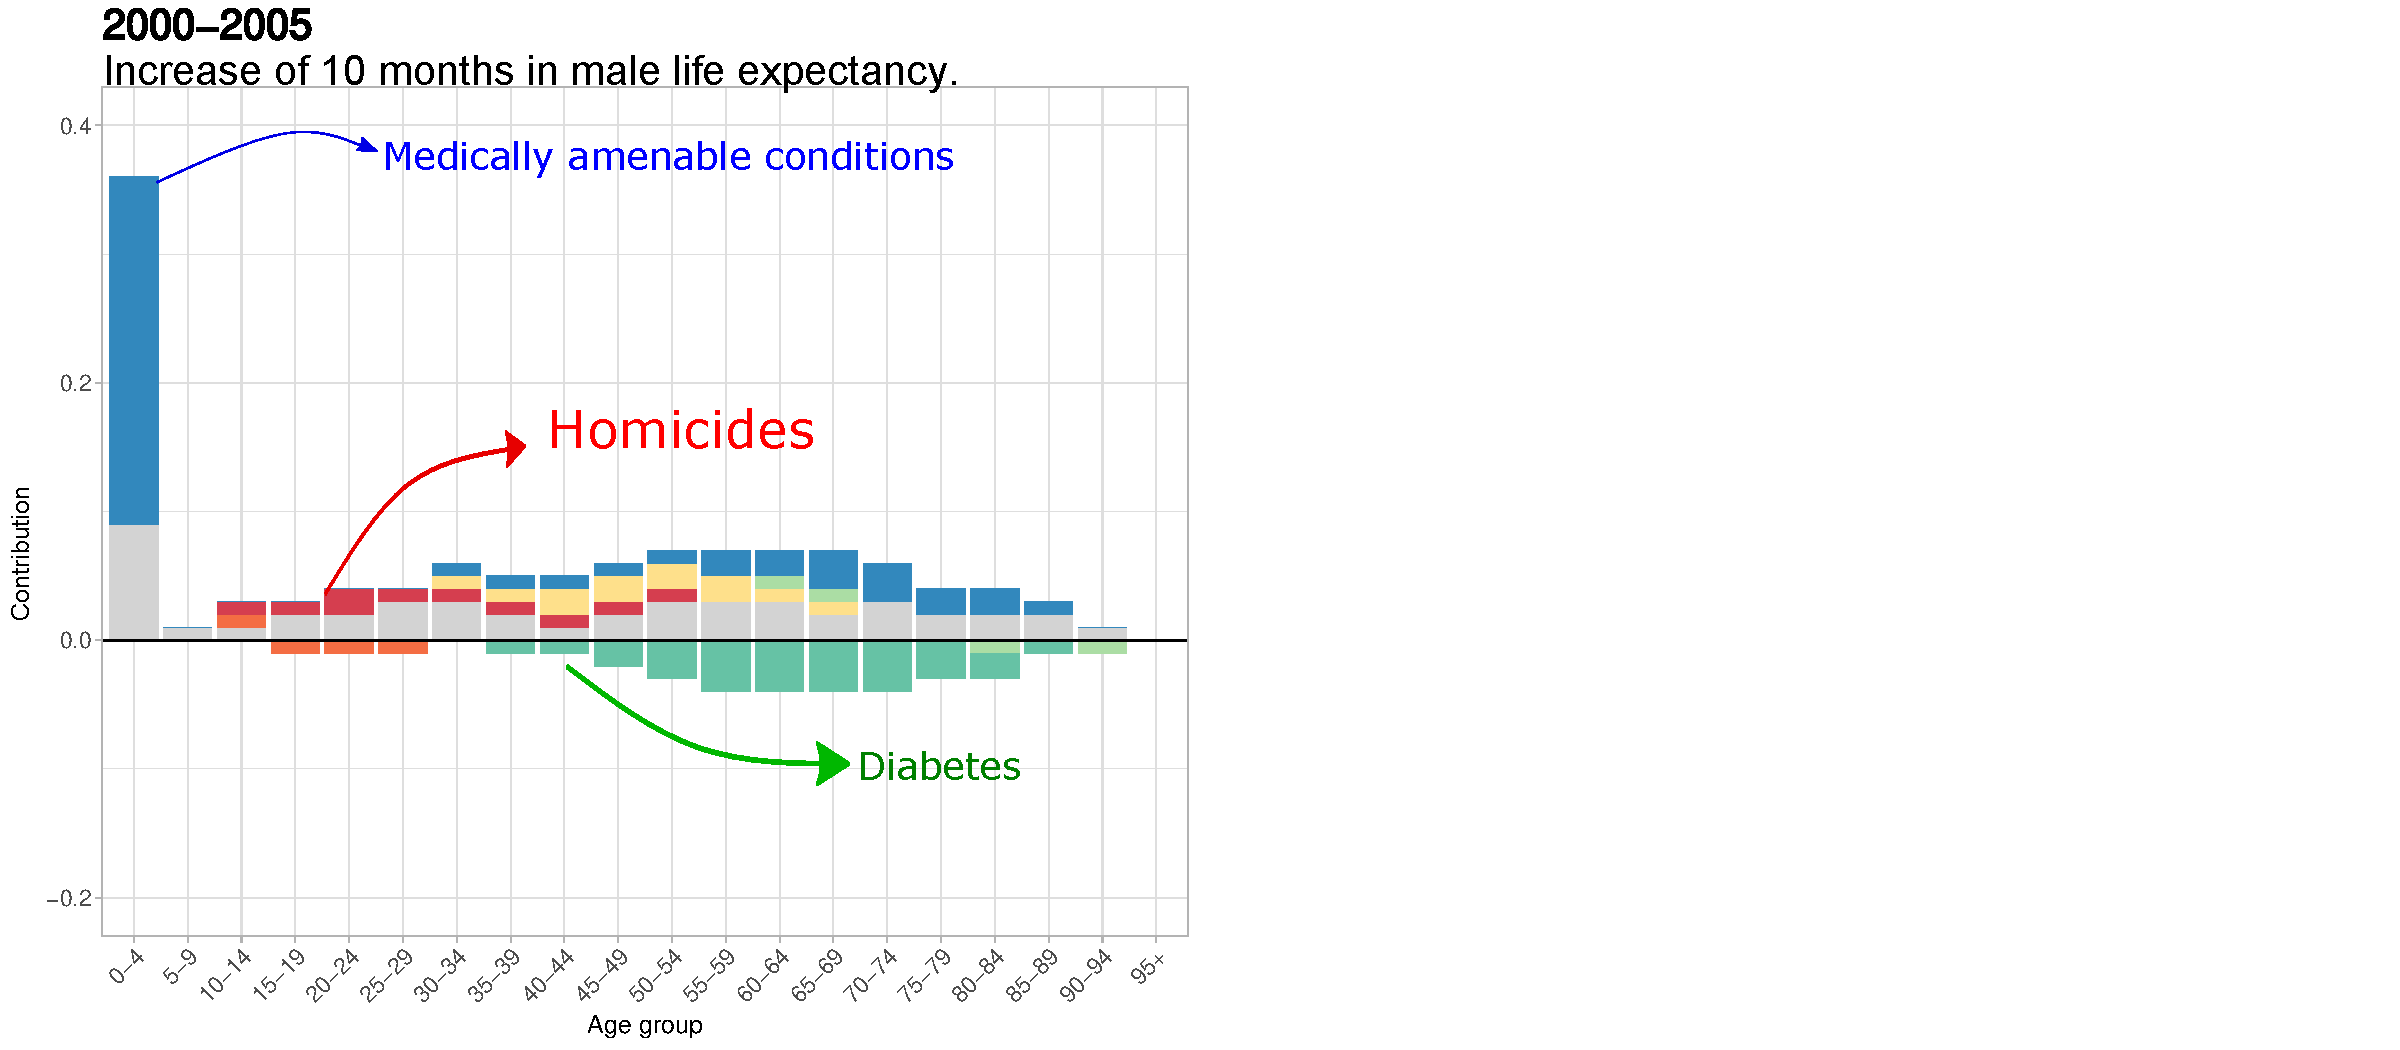
\includegraphics[scale=.31]{Figures/Fig2_1}
	
	\begin{center}
		\color{white}		\Large{\textbf{In 2005-2010 rates more than doubled}\\
		 (9.5 $\longrightarrow$ 22).}
	\end{center}	

\end{frame}


\begin{frame}
	\begin{center}
		\Large{In Mexico: homicides declined in 2000-2005}
	\end{center}

	
	\hspace*{-1cm}   
	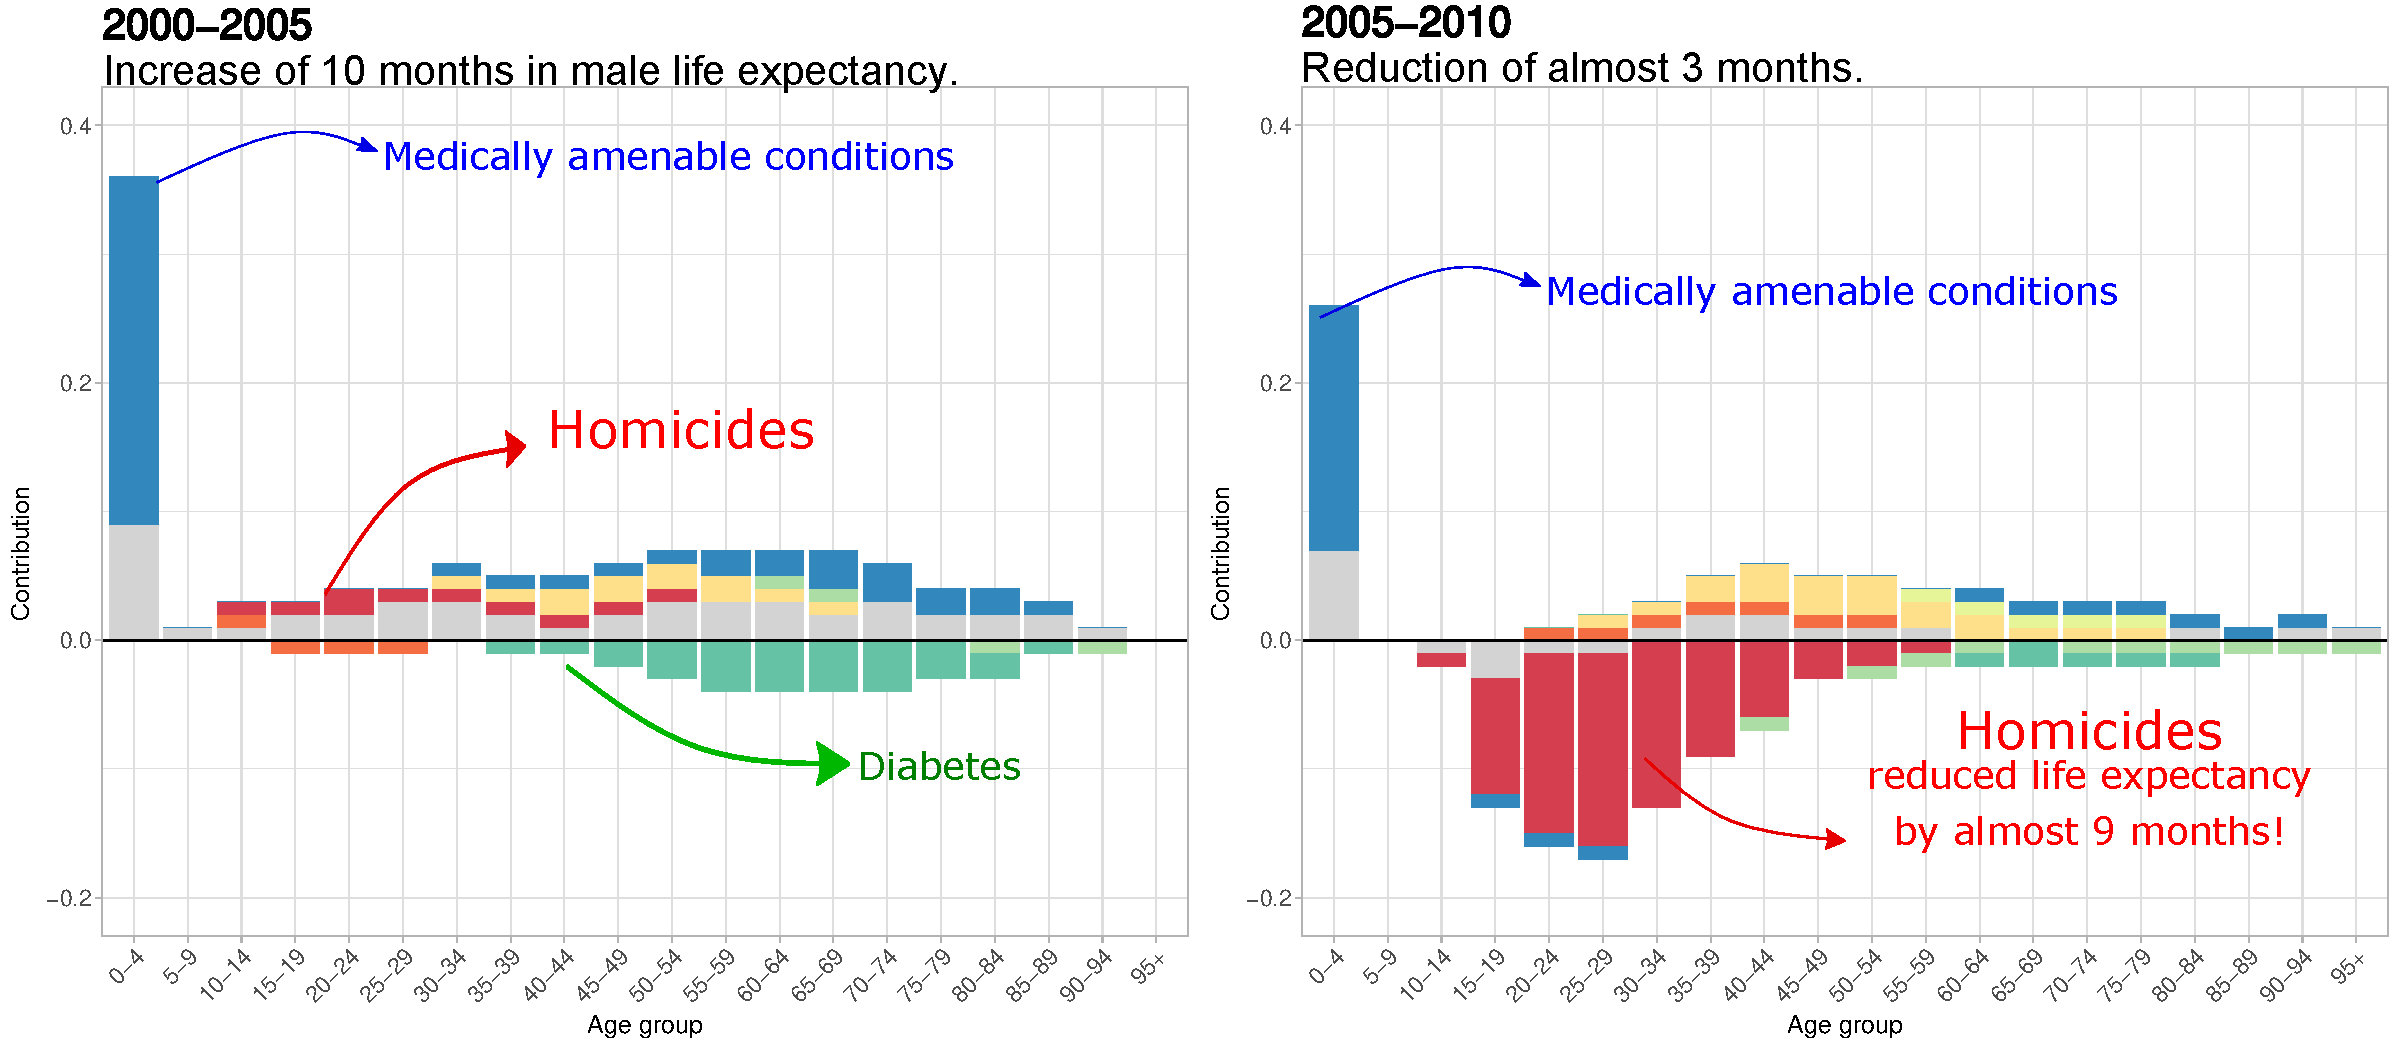
\includegraphics[scale=.31]{Figures/Fig2_2}
	
	\begin{center}
		\Large{\textbf{In 2005-2010 rates more than doubled}\\
		 (9.5 $\longrightarrow$ 22).}
	\end{center}	

\end{frame}



\begin{frame}
	\begin{center}
		\Large{	As a result, male life expectancy \textbf{stagnated} in the first decade of the new century ($\backsim 	$71y)}
	\end{center}
		
	\begin{center}
		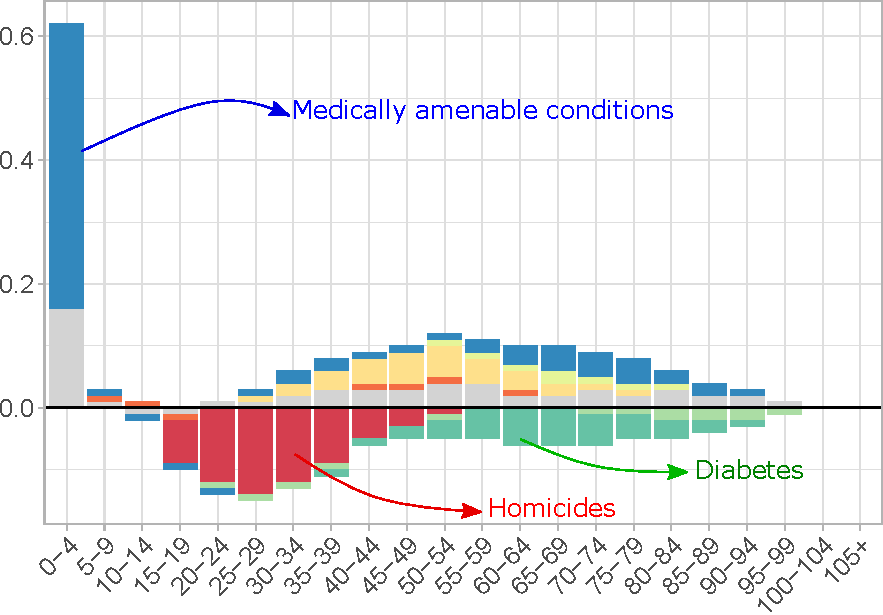
\includegraphics[scale=.65]{Figures/Fig_1}
	\end{center}

	\tiny{Canudas-Romo et al 2014}
	
\end{frame}



\begin{frame}
	\huge{
	\begin{center}
		\bf{Why did Mexico become so violent?}
	\end{center}
	}
	
	\pause
	
	\LARGE{
		\begin{itemize}
		
			\item \textbf{Competition} between drug cartels for territory. \pause
		
			\item \textbf{Enforcement operations} trying to mitigate drug trafficking operations after 2005. \pause
		
    	    \item \textbf{Increased profitability} in the drug-trade flow with United States. 
		
		\end{itemize}
		
	\tiny{Sources: Rios 2013, Dell 2015, Castillo et al 2014}
	}

\end{frame}



\begin{frame}

	\begin{center}
		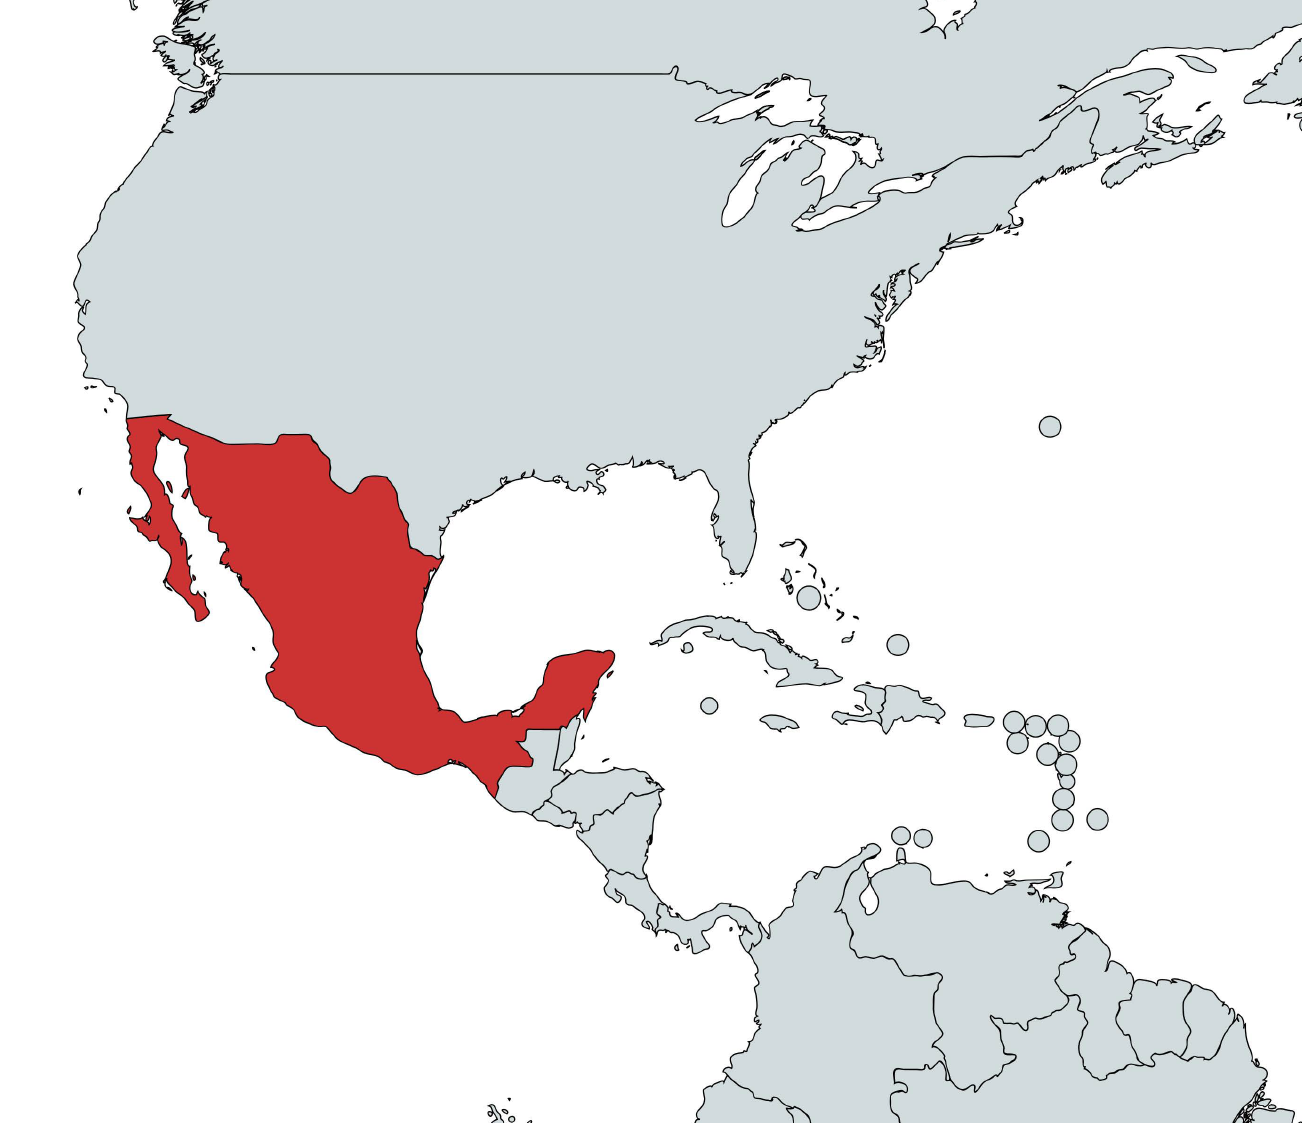
\includegraphics[scale=.3]{Figures/Mexico1}
	\end{center}
				
\end{frame}



\begin{frame}
	\huge{
	\begin{center}
		\bf{Propagation of violence}\linebreak
	\end{center}
		}

	\begin{center}		
		\animategraphics[autoplay, scale=0.17]{1}{Figures/Propagation}{0}{5}
	\end{center}

	\tiny{Espinal-Enriquez \& Larralde 2015}
\end{frame}



\begin{frame}
	\Large{Changes in male life expectancy at birth by state}


	\begin{center}
		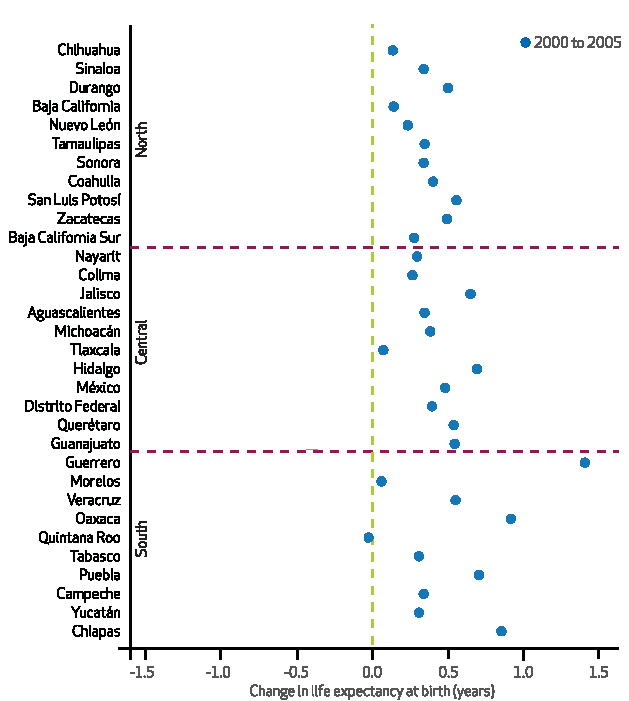
\includegraphics[scale=.66]{Figures/Changes_states_1}
	\end{center}
	
	\tiny{Aburto et al. 2016}				
\end{frame}

\begin{frame}
	\Large{Changes in male life expectancy at birth by state}


	\begin{center}
		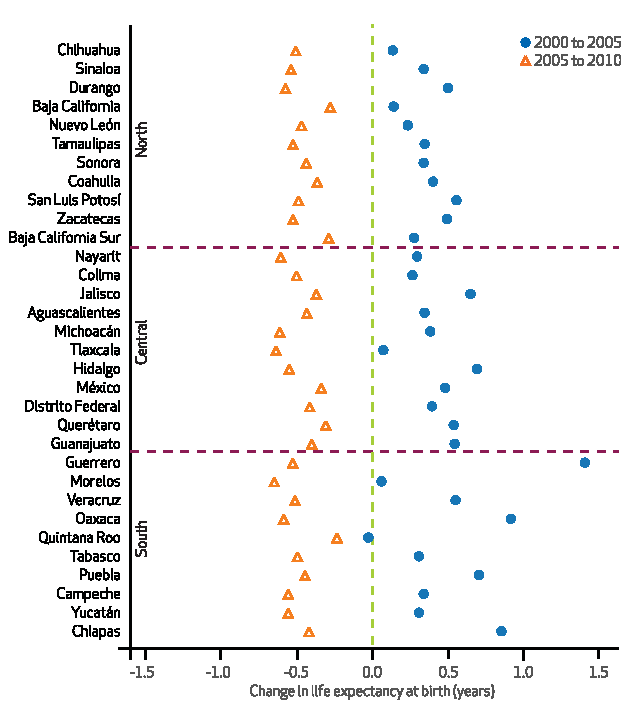
\includegraphics[scale=.66]{Figures/Changes_states_2}
	\end{center}
	
	\tiny{Aburto et al. 2016}				
\end{frame}



\begin{frame}
	\begin{center}
		\Large{Homicide contribution to changes in male life expectancy at birth by state}
	\end{center}

	\begin{center}
		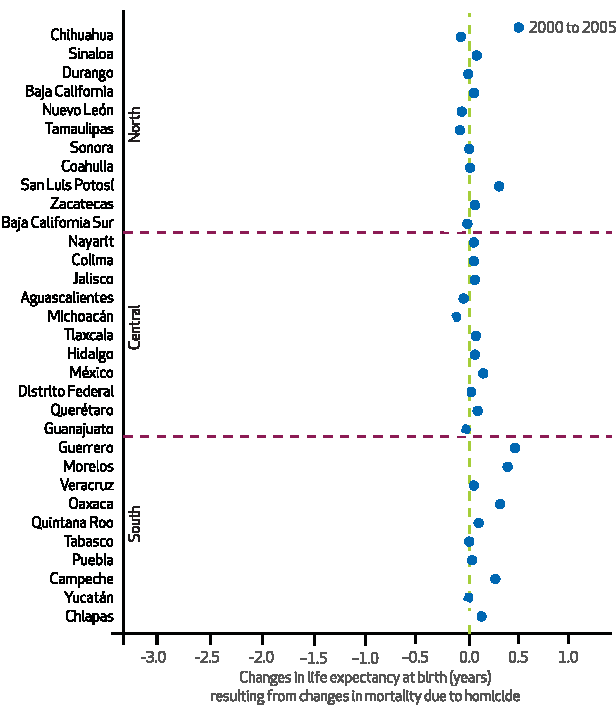
\includegraphics[scale=.62]{Figures/State_homicides_1}
	\end{center}
	
	\tiny{Aburto et al. 2016}				
\end{frame}


\begin{frame}
	\begin{center}
		\Large{Homicide contribution to changes in male life expectancy at birth by state}
	\end{center}


	\begin{center}
		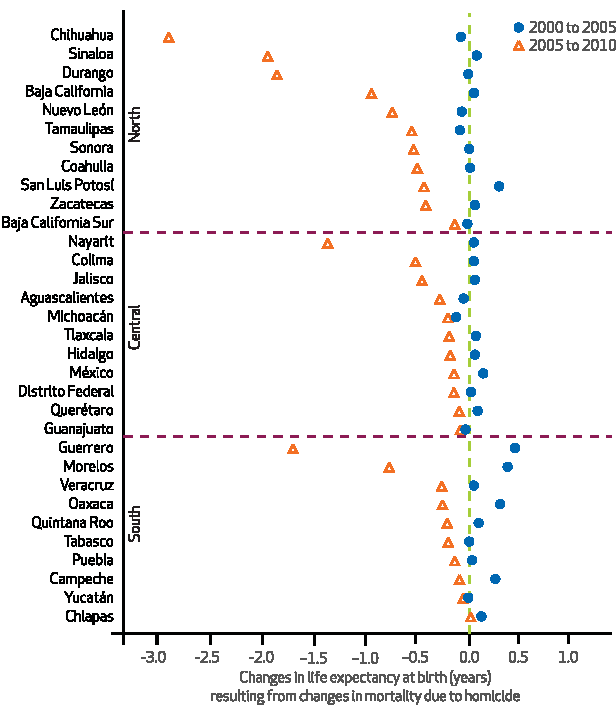
\includegraphics[scale=.62]{Figures/State_homicides_2}
	\end{center}
	
	\tiny{Aburto et al. 2016}				
\end{frame}

\begin{frame}
	\LARGE{

		\begin{center}		
			\textbf{Gains in life expectancy} due to medically amenable causes
		\end{center}
		
		\begin{enumerate}
			\item Infectious
			\item Respiratory diseases 
			\item Birth conditions
			\item ...
		\end{enumerate}

	\pause

	\begin{center}
		\textbf{Wiped out by the increase of homicides between 2005-10 in each of the 32 states in Mexico}
	\end{center}				
	\tiny{Aburto et al. 2016}			
}
\end{frame}


%
%
%\begin{frame}
%	\LARGE{
%		\begin{center}
%			\textbf{Consequences of violence go beyond homicides}
%		\end{center}
%	
%	\pause
%	
%	Victims of violence
%	\begin{itemize}
%		
%		\item Depression
%
%		\item Alcohol abuse
%		
%		\item Suicidal behavior
%		
%		\item Psychological problems
%						
%	\end{itemize}	
%	
%		}
%		\tiny{Davidson et al. 1996,Braveman et al 2014,Mikton et al. 2014}
%\end{frame}
%%
%\begin{frame}
%	\LARGE{
%		\begin{center}
%			\textbf{Consequences of violence go beyond homicides}
%		\end{center}
%	
%	Witnessing violence
%	
%		\begin{itemize}
%		
%		\item Higher rates of post-traumatic stress disorder
%
%		\item Depression 
%		
%		\item Externalize violence
%		
%		\item \textbf{Perceived vulnerability (fear)} 
%						
%	\end{itemize}
%	
%		}
%		\tiny{Buka et al. 2001}
%\end{frame}
%
%
%\begin{frame}
%	\LARGE{
%		\begin{center}	
%		\textbf{Aim: To estimate the average number of years spent vulnerable of becoming victims of violence}
%		\end{center} 
%		
%		\pause
%		
%		\begin{enumerate}
%		
%		\item Surveys of perception of public safety.
%
%		\item Mortality data.
%		
%		\item Sullivan method.
%		
%						
%		\end{enumerate}
%	
%		}
%		\tiny{Canudas-Romo et al 2017}
%\end{frame}
%
%\begin{frame}
%	\Large{
%	\begin{center}
%			\textbf{Mexican life expectancy with and without vulnerability, 2005 and 2014.}
%	\end{center}
%	
%	\begin{center}
%		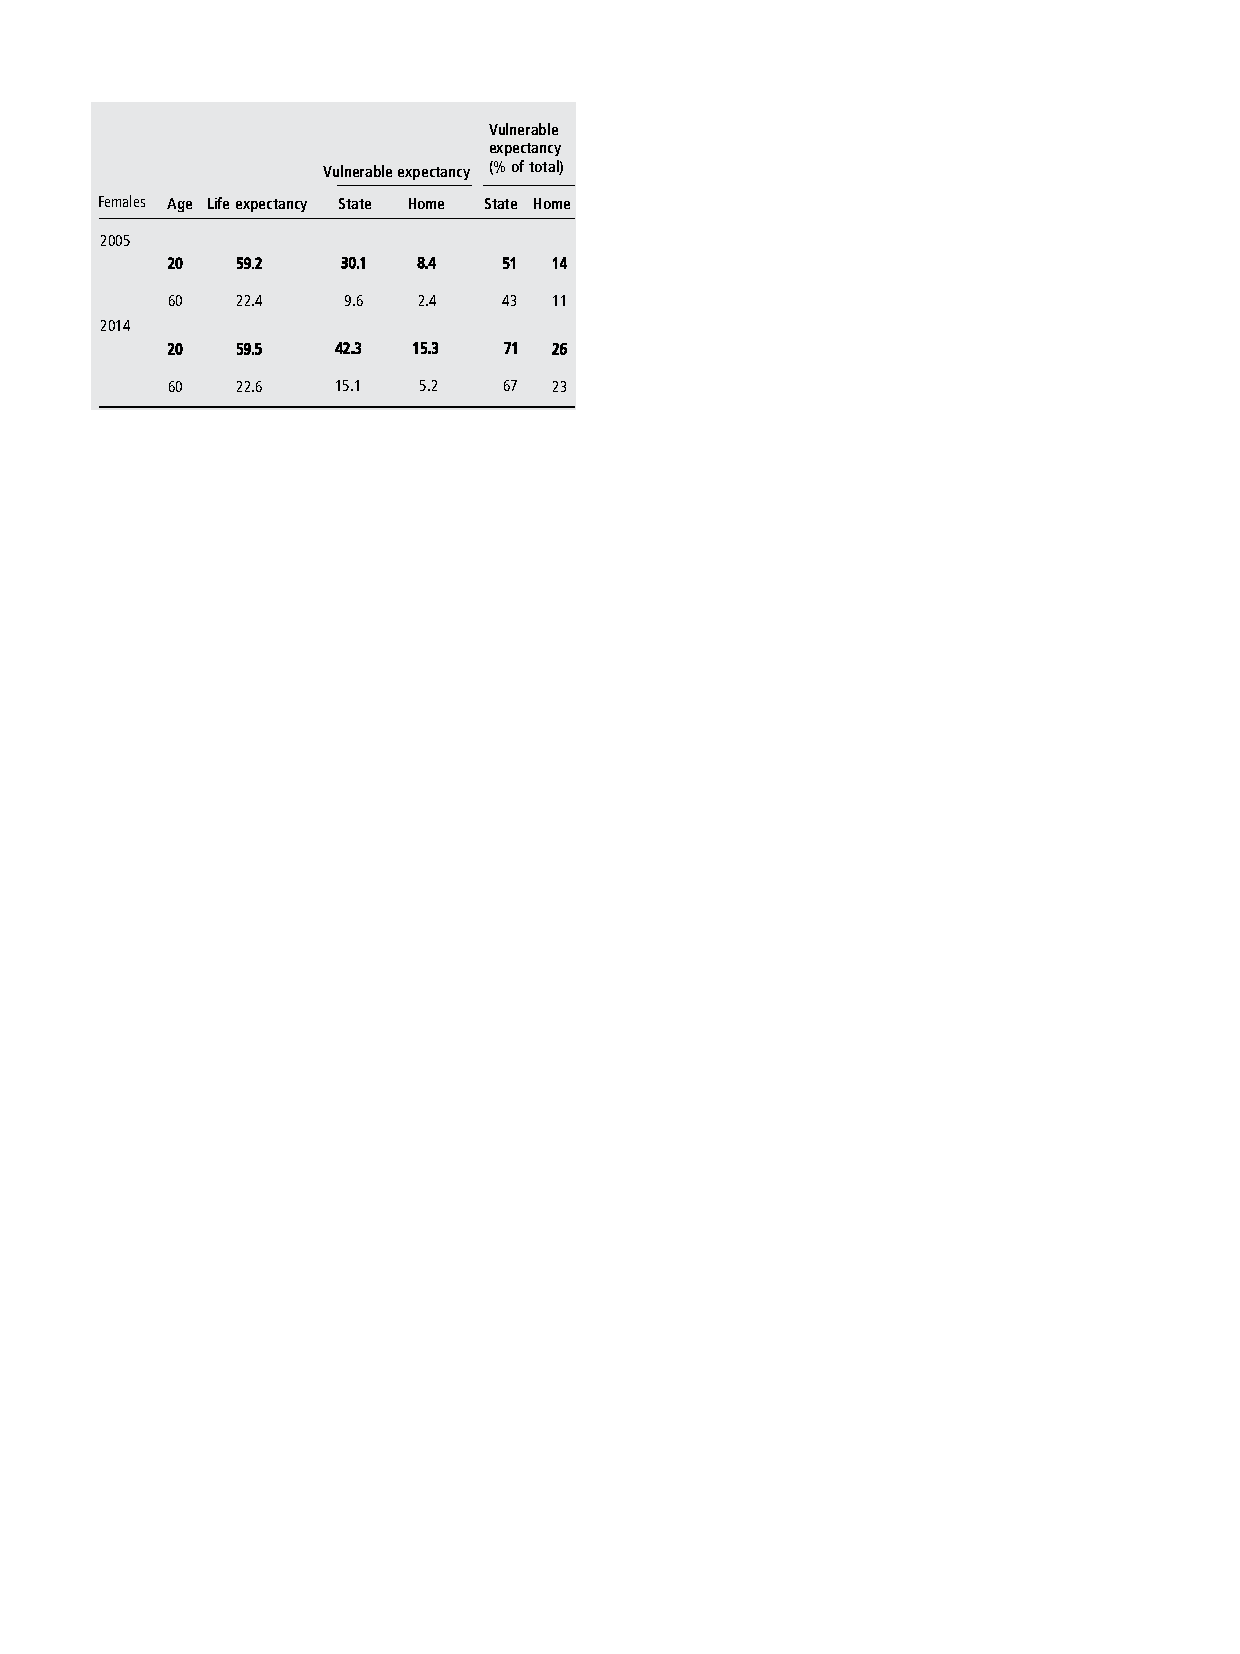
\includegraphics[scale=1.2]{Figures/Vulnerability}
%		
%		\pause
%		
%		\textbf{Increase of 30.5 million person-years.}
%	\end{center}
%		}
%		
%		\tiny{Canudas-Romo et al 2017}
%\end{frame}


\begin{frame}
	\huge{
		\begin{center}
		
		\textbf{What is the effect of homicides on the uncertainty of life?}
		
		\end{center}		

	}
\end{frame}

\begin{frame}
	\begin{center}
		\Large{\textbf{What is lifespan variation or lifespan inequality?}}
	\end{center}


	\begin{center}
		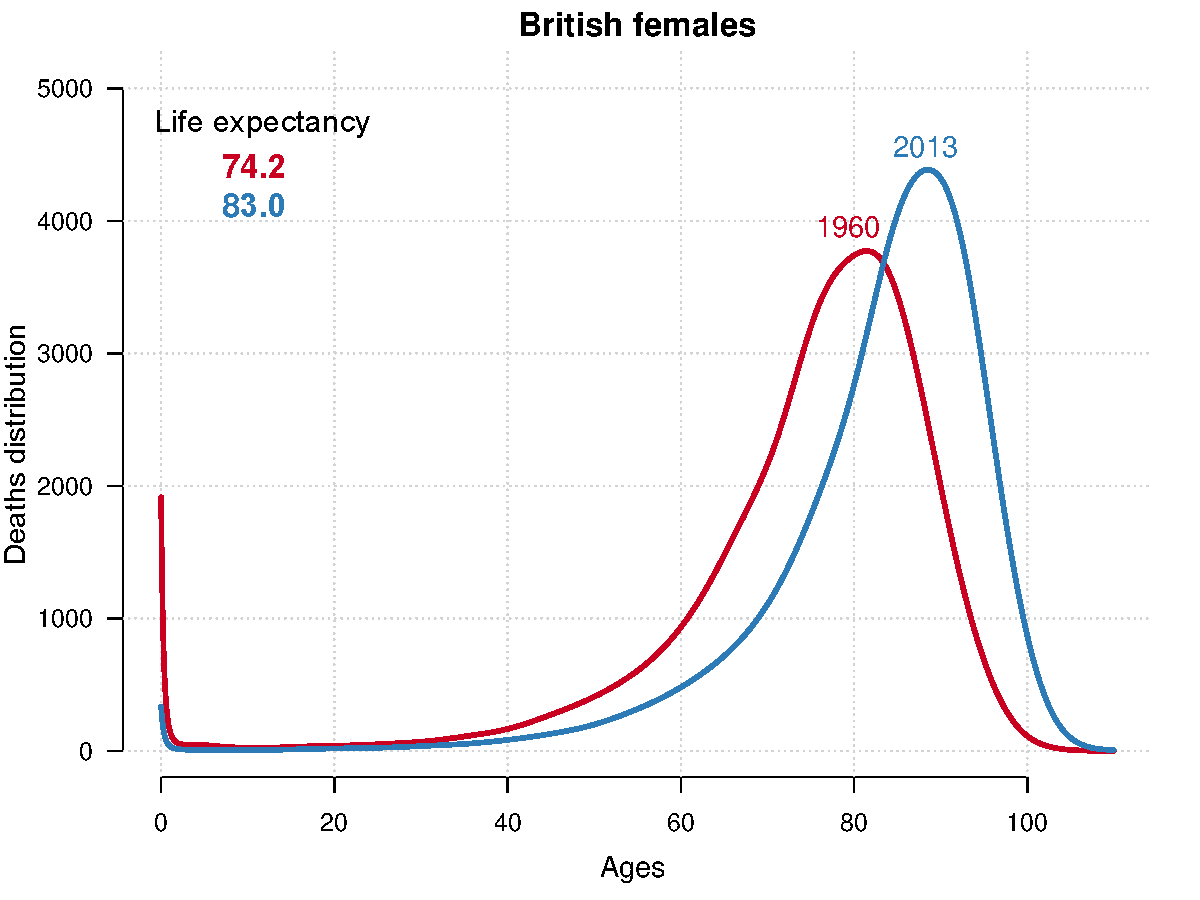
\includegraphics[scale=.49]{Figures/DistribGBR1}
	\end{center}
	
\end{frame}

\begin{frame}
	\begin{center}
		\Large{\textbf{What is lifespan variation or lifespan inequality?}}
	\end{center}


	\begin{center}
		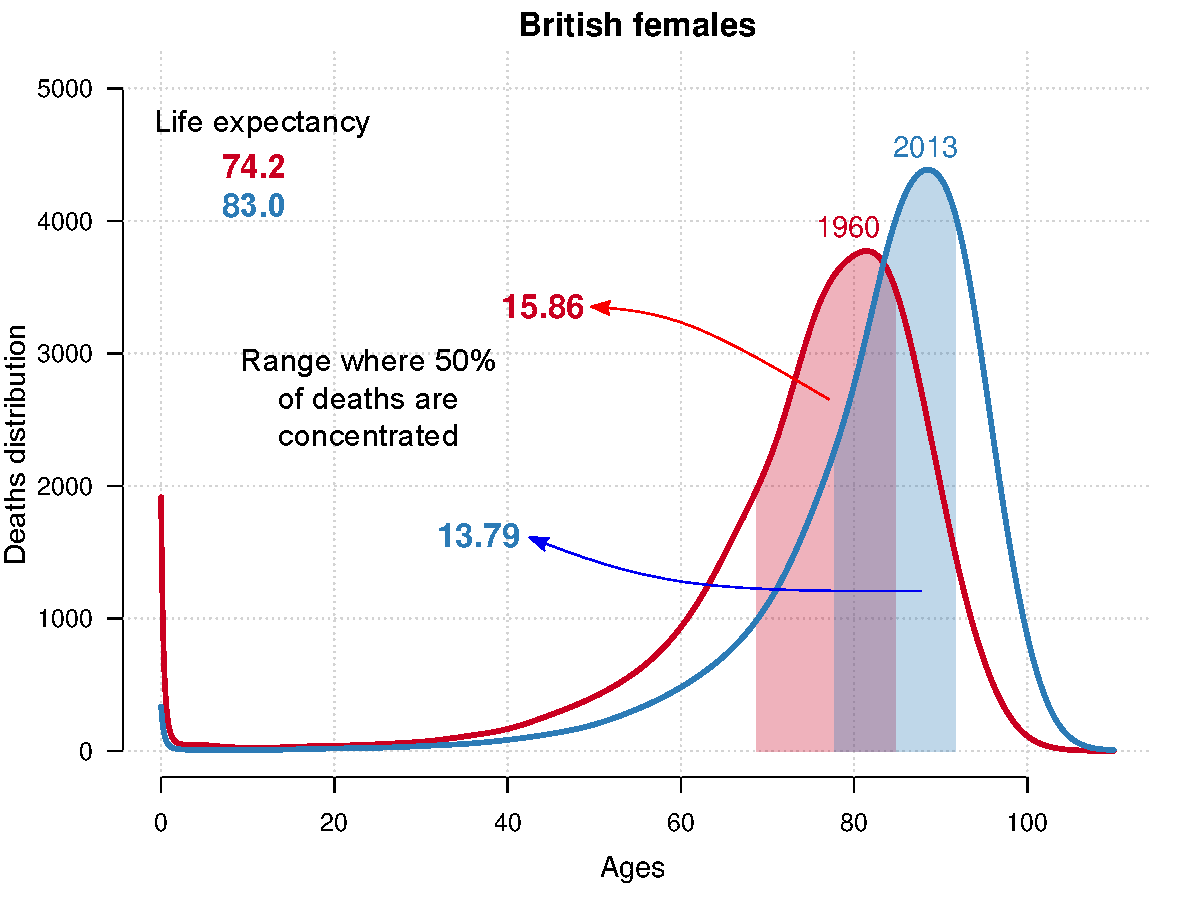
\includegraphics[scale=.49]{Figures/DistribGBR2}
	\end{center}
			
\end{frame}

\begin{frame}
\LARGE{
\textbf{Why lifespan variation?}
		\begin{itemize}
		
		\item Greater \textbf{uncertainty} in the timing of death. \pause

		\item Implications on \textbf{planning} of life's events. \pause
		
		\item \textbf{Increasing} vulnerability at the societal level. \pause
		
		\item \textbf{Ineffectiveness} of policies aiming to protect individuals.
						
		\end{itemize}

}
\end{frame}


\begin{frame}

\Large{
	\textbf{$e^{\dagger}_{15}\longrightarrow  $} Life lost when death occurs.

	\begin{itemize}
		\item Easy \textbf{public health interpretation}.
		\pause
		\item \textbf{Quantify} age and cause specific effects.
		\pause
		\item Separate ages that \textbf{decrease} from those that \textbf{increase}.
		\pause
		\item Conditioned to age 15 to capture the \textbf{onset of violence}.
	\end{itemize}

}
\end{frame}



\begin{frame}
	\begin{center}
		\Large{\textbf{National lifespan inequality}}
	\end{center}

	\hspace*{-1cm}   
	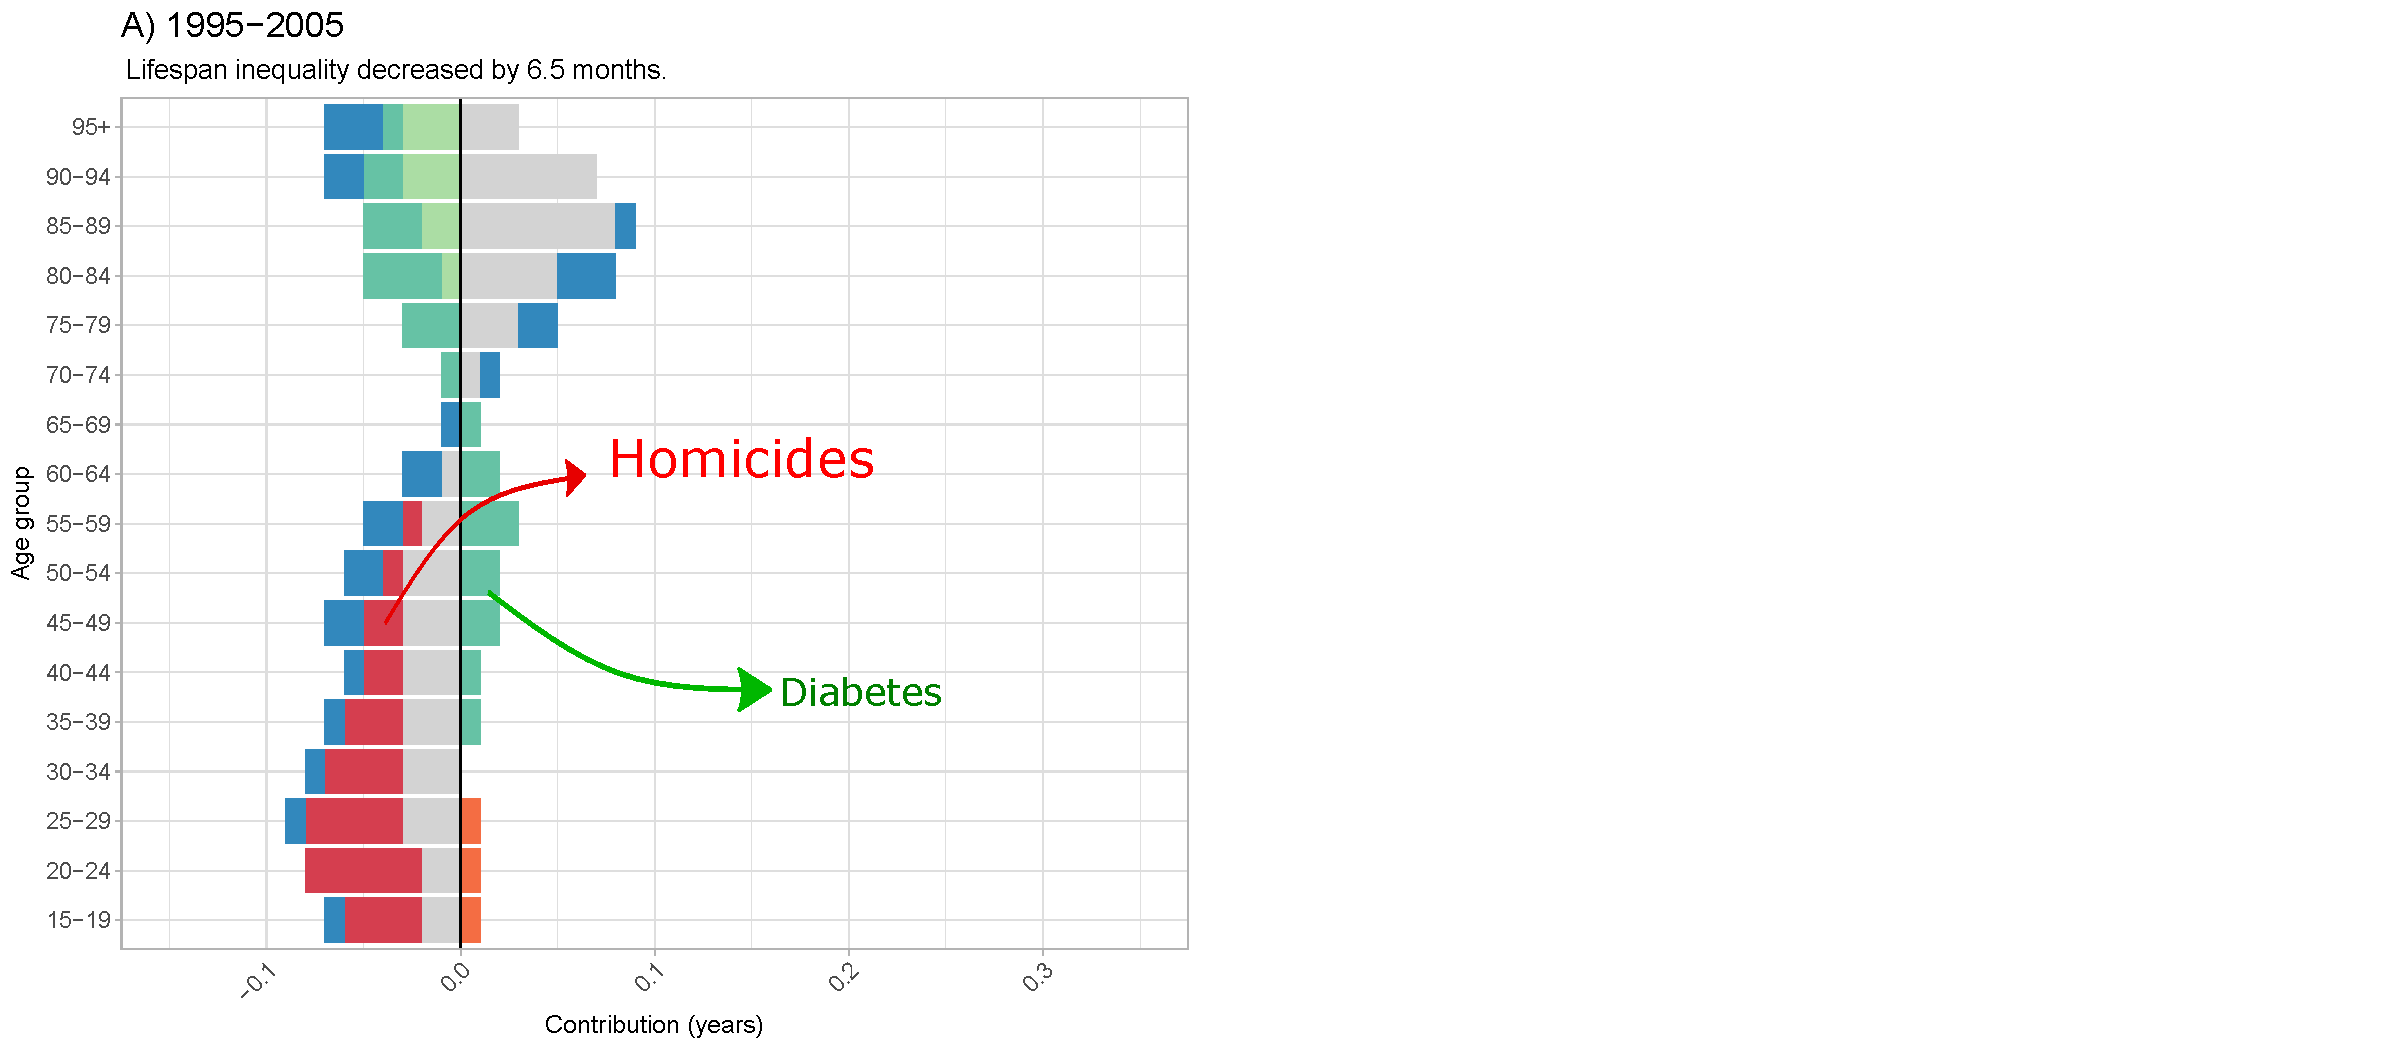
\includegraphics[scale=.31]{Figures/Figure_2_2}
	
\end{frame}


\begin{frame}
	\begin{center}
		\Large{\textbf{National lifespan inequality}}
	\end{center}

	\hspace*{-1cm}   
	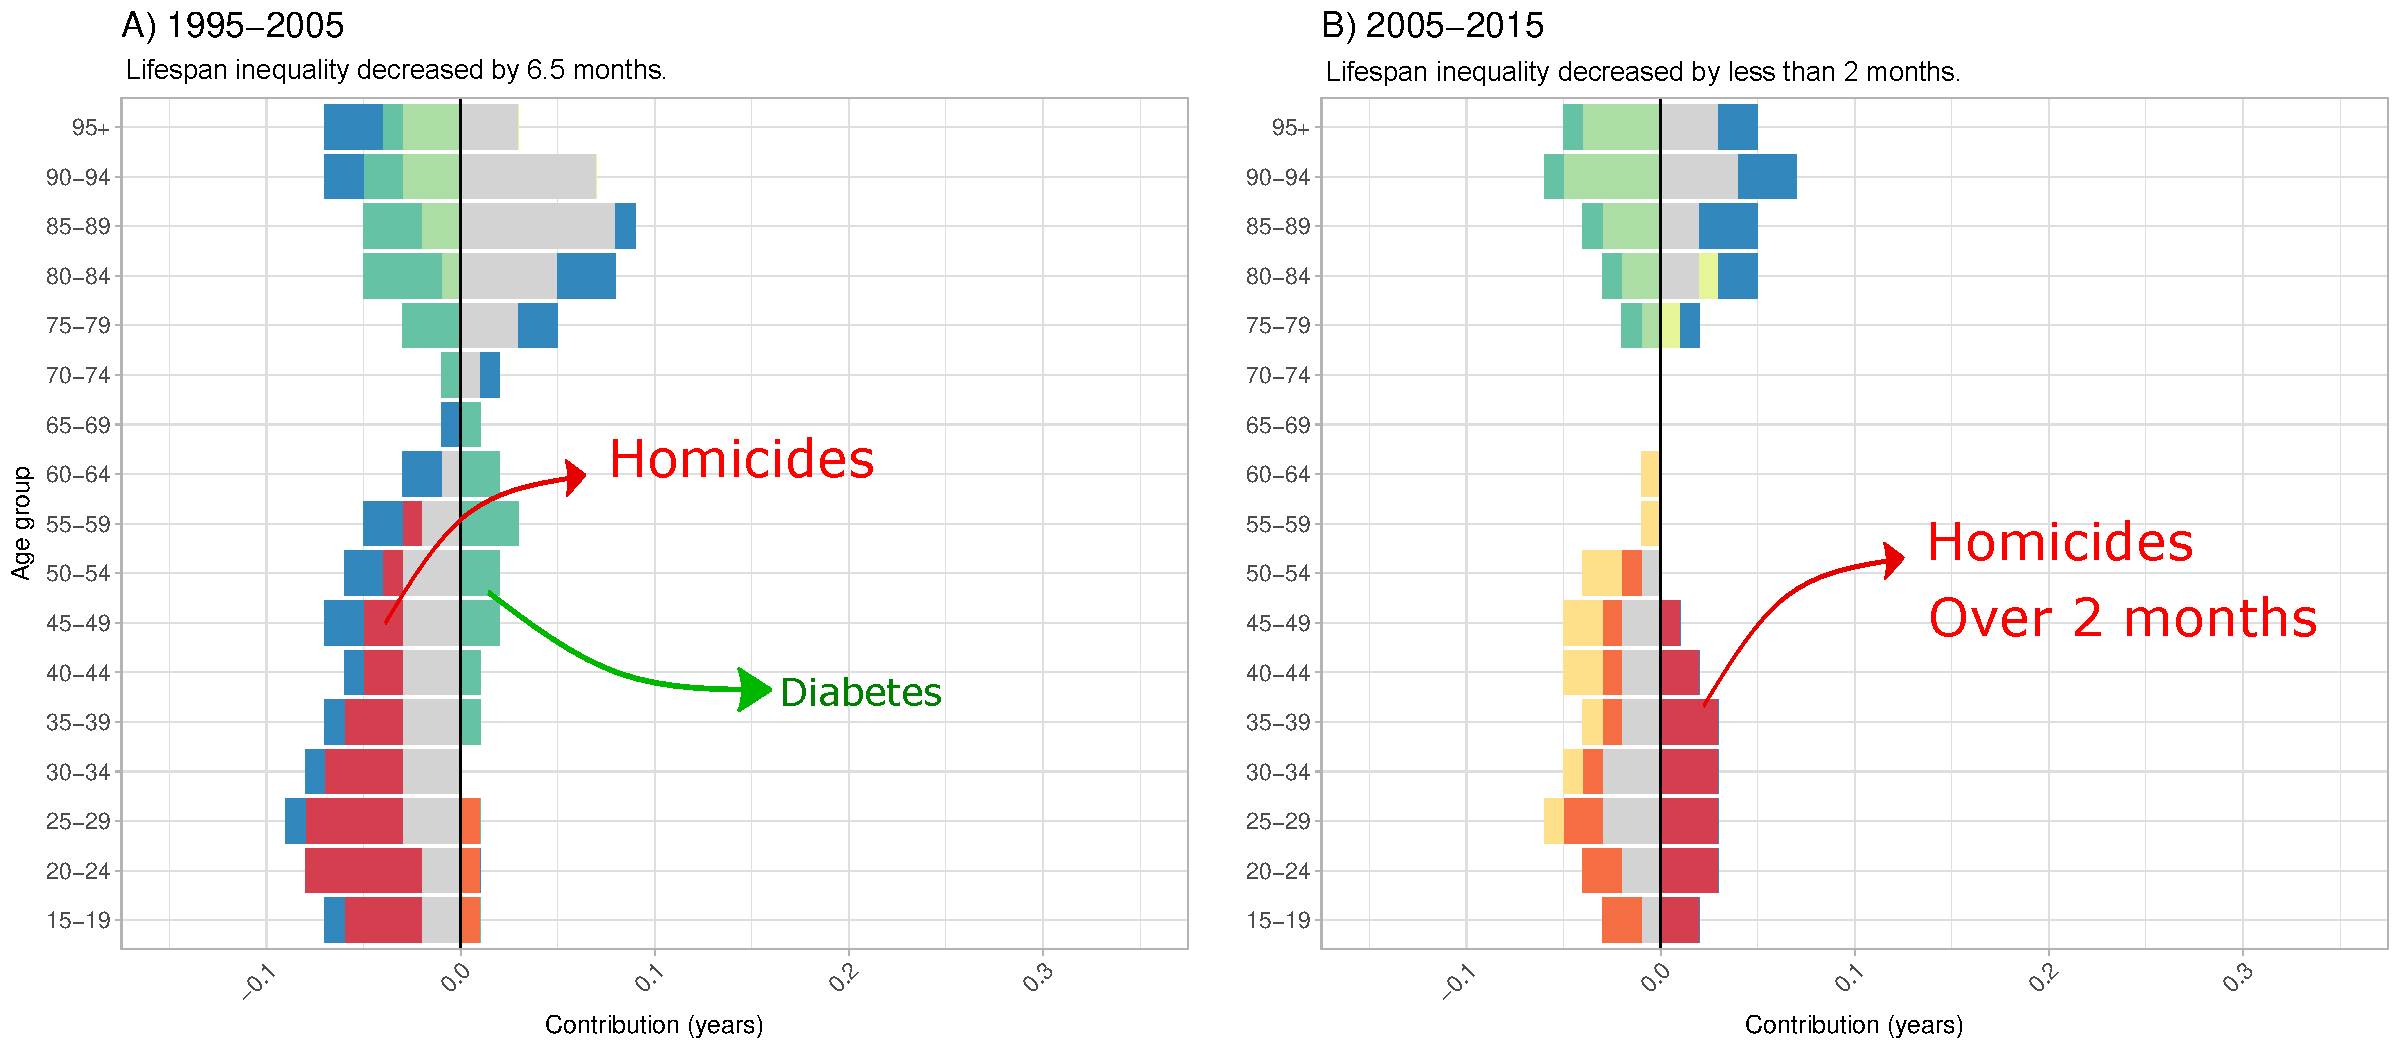
\includegraphics[scale=.31]{Figures/Figure_2}	

\end{frame}


\begin{frame}
	\begin{center}
		\Large{\textbf{Changes in male lifespan inequality by state}}

		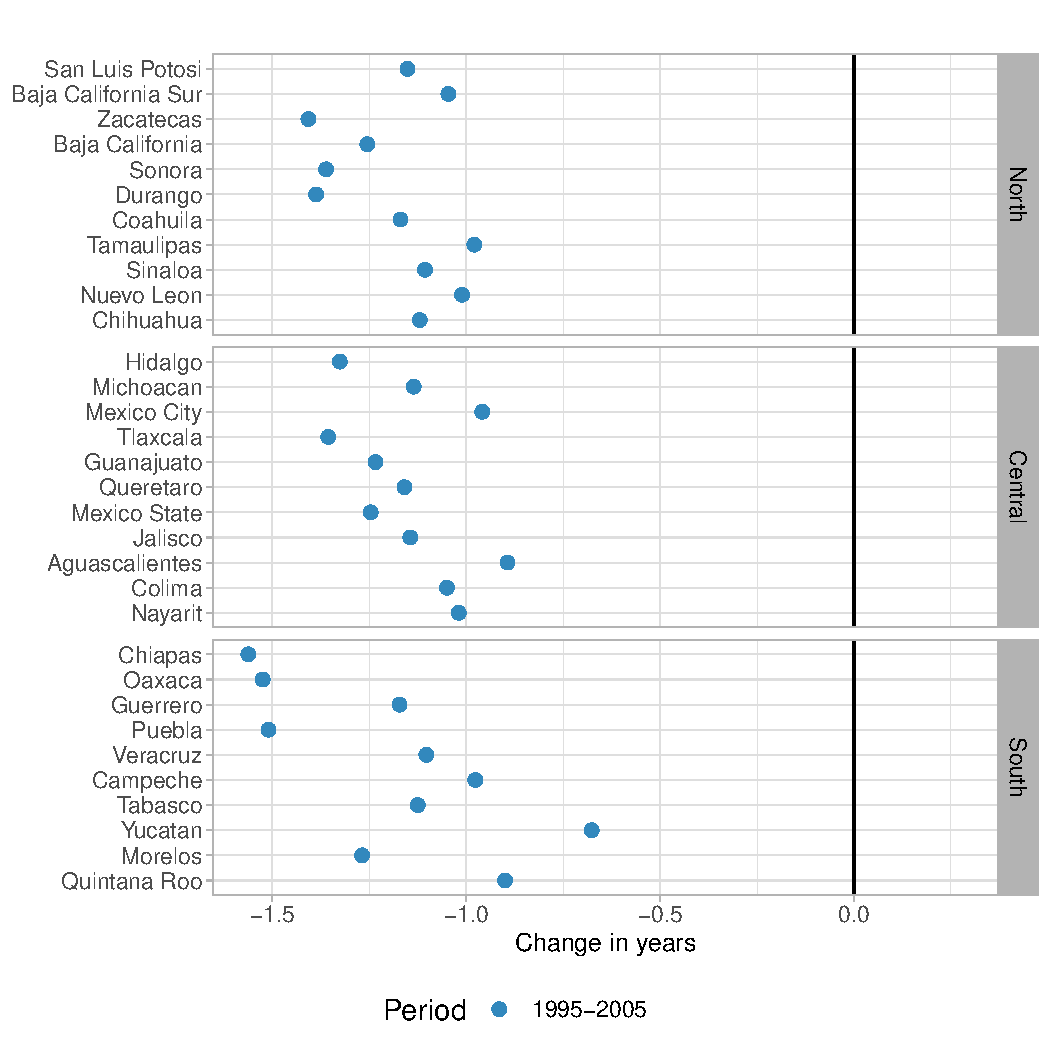
\includegraphics[scale=.47]{Figures/Figure_3_1}
		\end{center}

\end{frame}

\begin{frame}
	\begin{center}
		\Large{\textbf{Changes in male lifespan inequality by state}}

		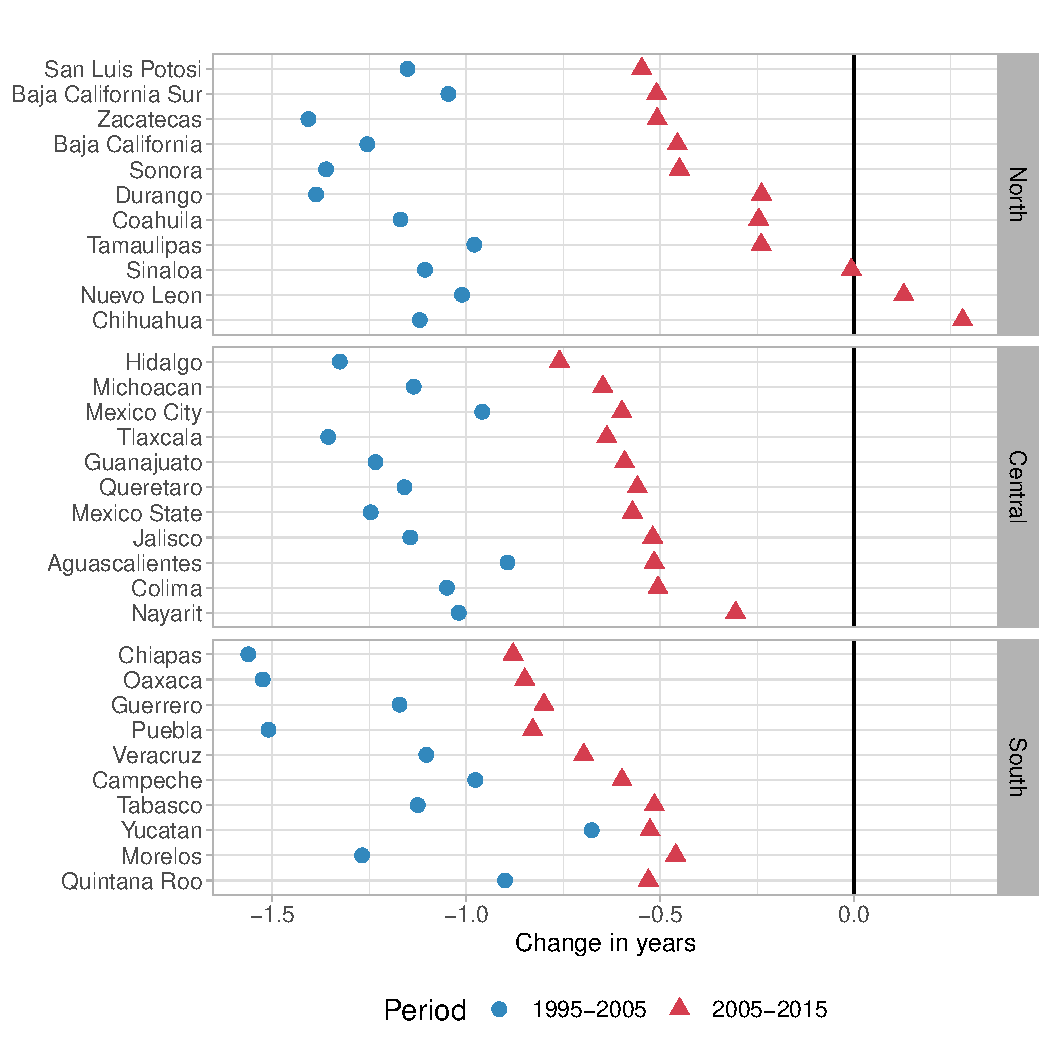
\includegraphics[scale=.47]{Figures/Figure_3}
		\end{center}

\end{frame}


\begin{frame}
	\begin{center}
		\Large{\textbf{Homicide contribution to lifespan inquality}}
		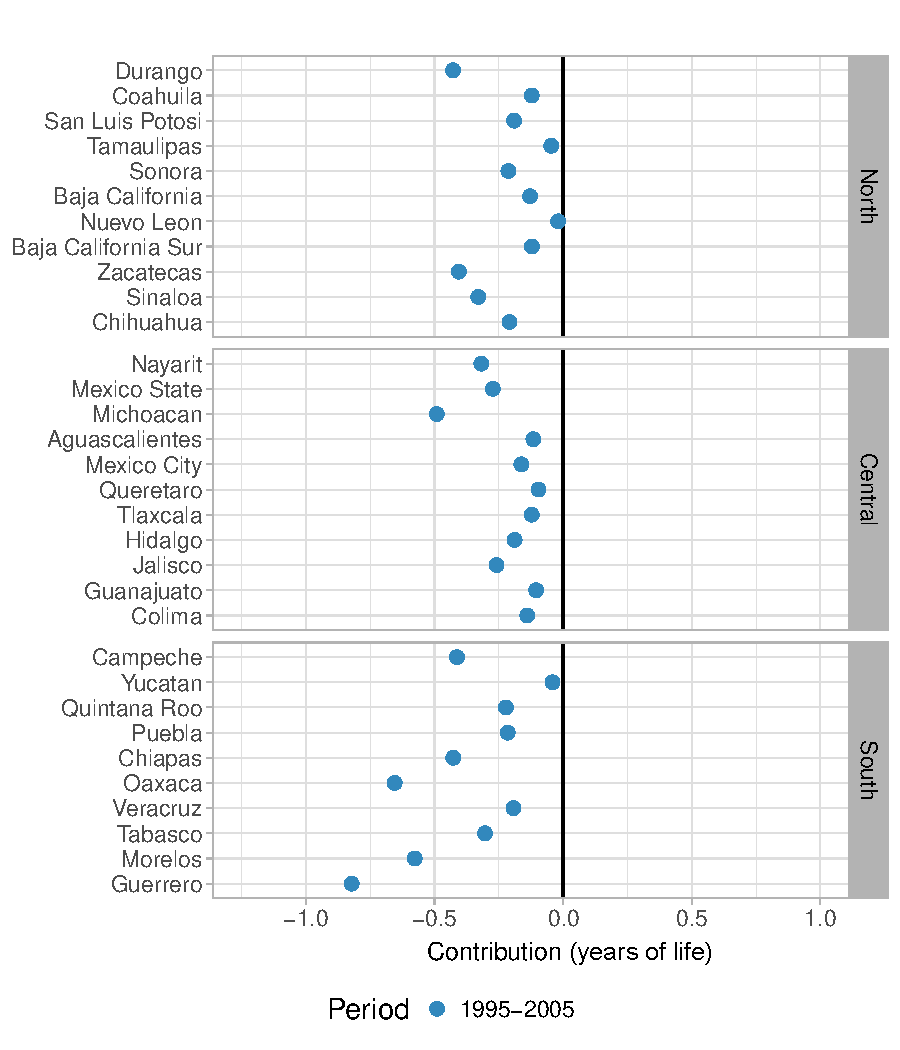
\includegraphics[scale=.47]{Figures/Figure_4_1}
	\end{center}

\end{frame}

\begin{frame}
	\begin{center}
		\Large{\textbf{Homicide contribution to lifespan inquality}}
		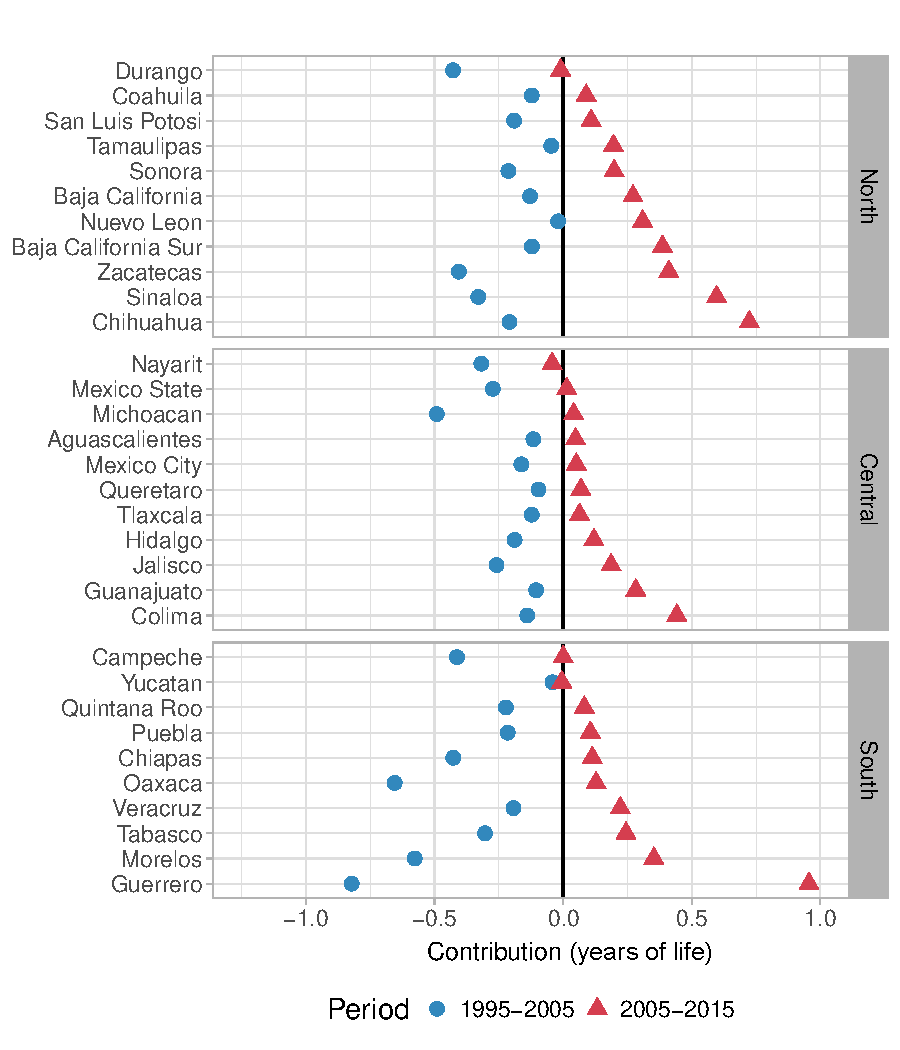
\includegraphics[scale=.47]{Figures/Figure_4}
	\end{center}

\end{frame}


\begin{frame}
	\begin{center}
		\Large{\textbf{Homicide contribution to lifespan inquality}}
		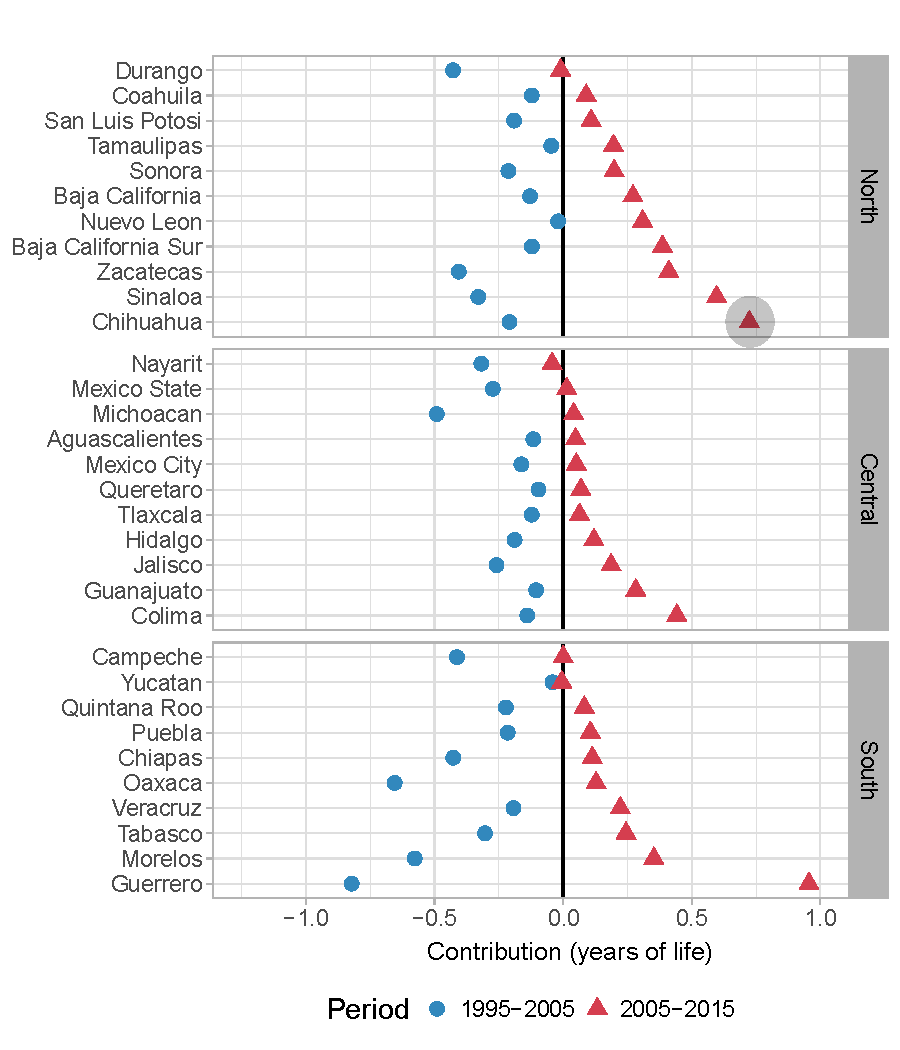
\includegraphics[scale=.47]{Figures/Figure_42}
	\end{center}

\end{frame}

\begin{frame}
	\begin{center}
		\Large{\textbf{Homicide contribution to lifespan inquality}}
		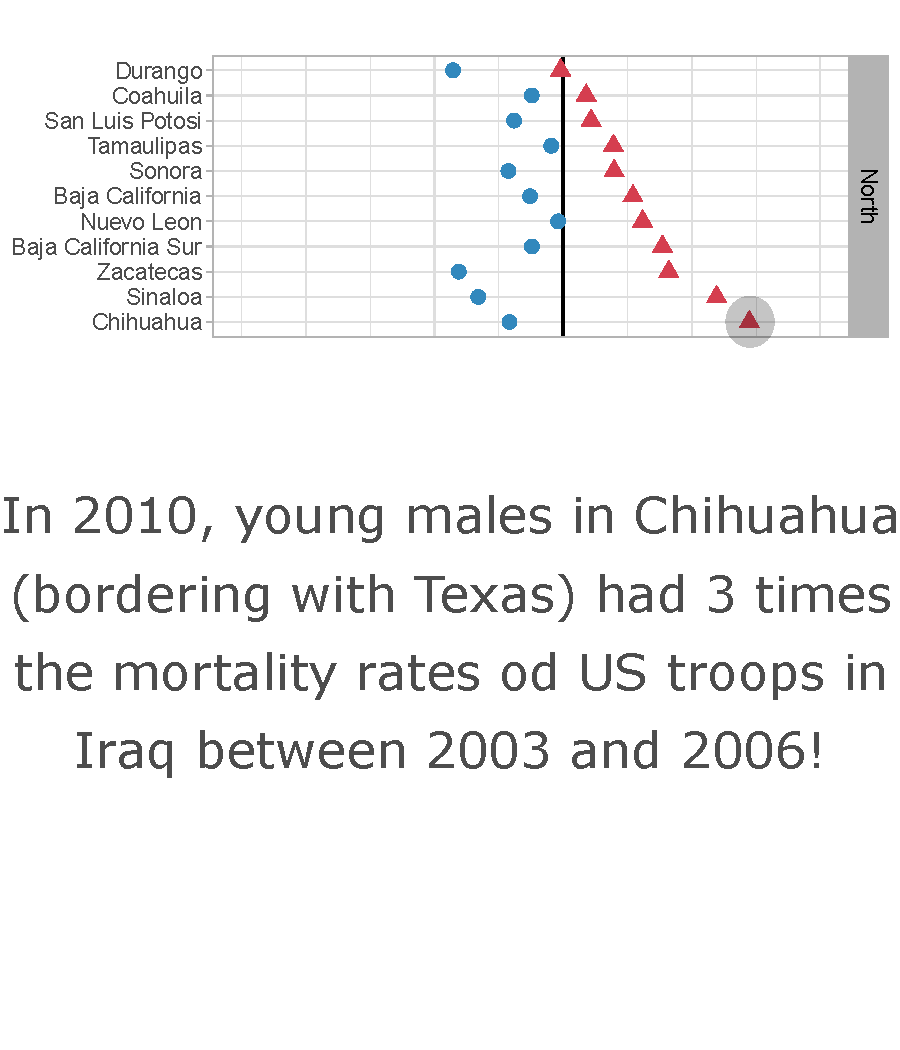
\includegraphics[scale=.47]{Figures/Figure_422}
	\end{center}

\end{frame}


\begin{frame}
	\begin{center}
		\Large{\textbf{Homicide contribution to lifespan inquality}}
		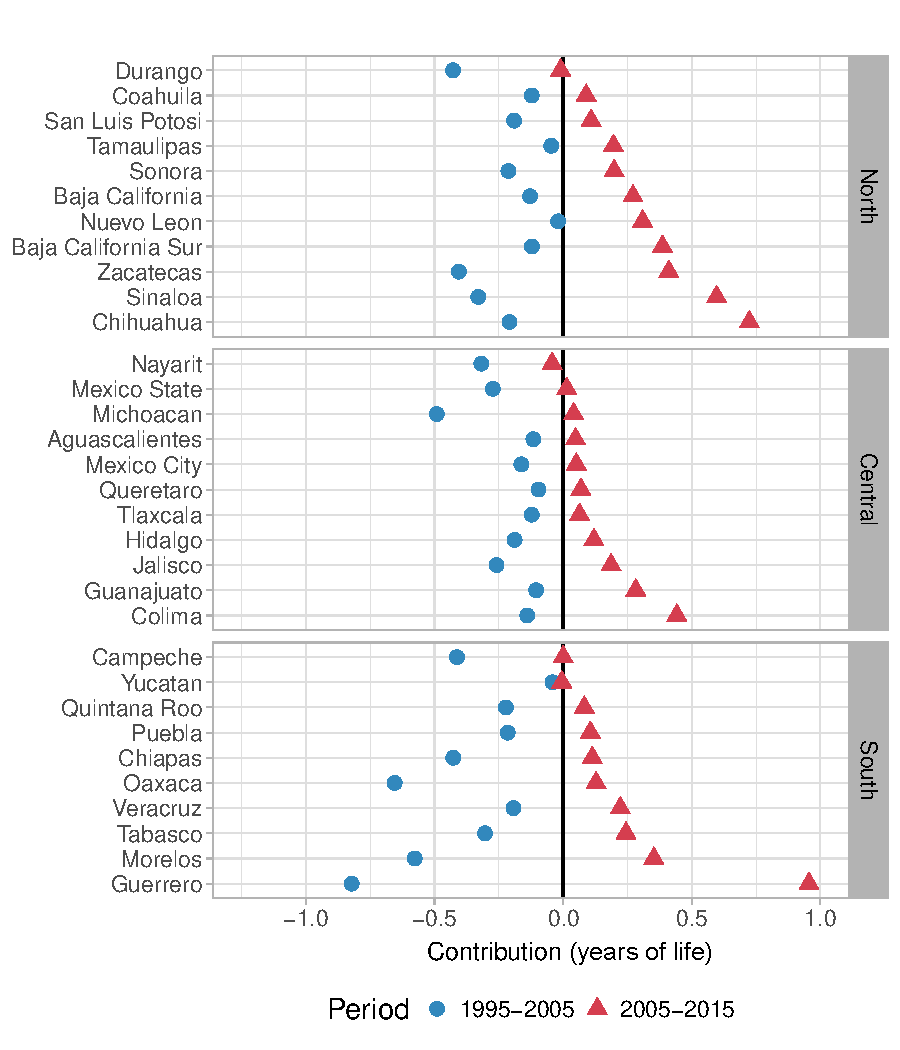
\includegraphics[scale=.47]{Figures/Figure_4}
	\end{center}

\end{frame}

\begin{frame}
	\begin{center}
		\Large{\textbf{Homicide contribution to lifespan inquality}}
		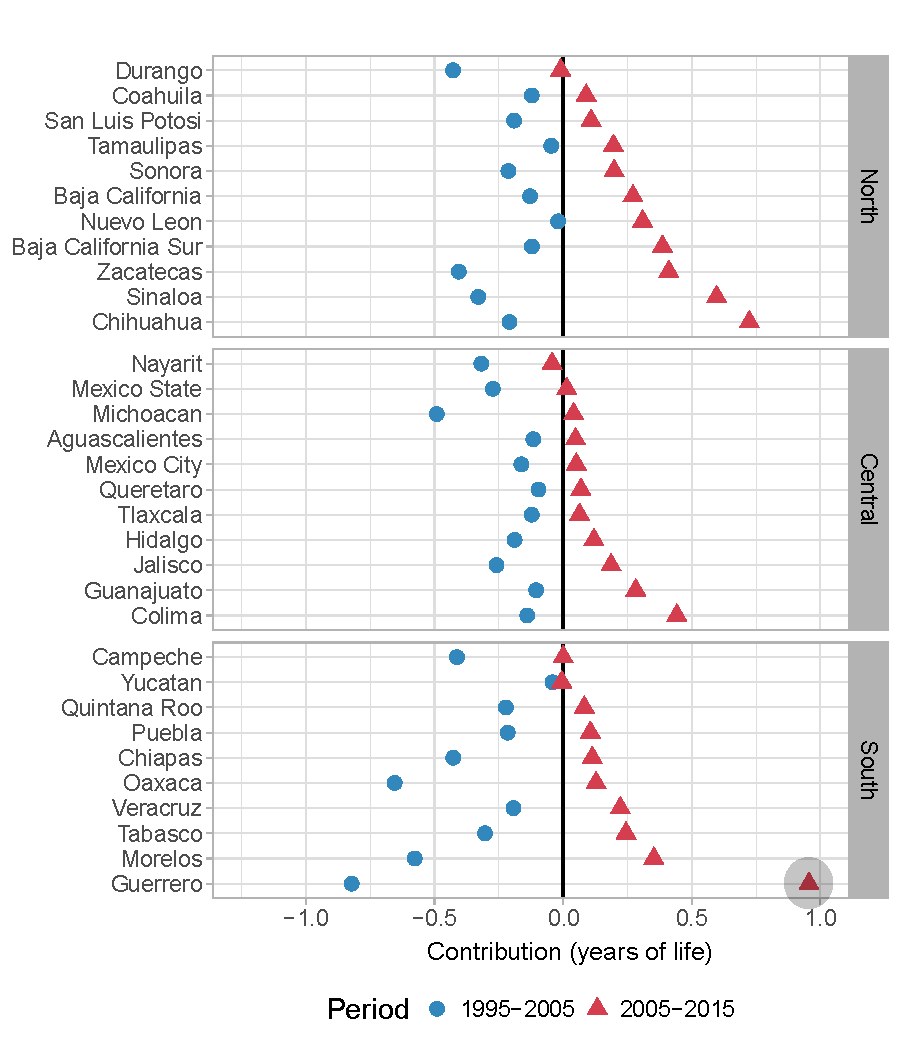
\includegraphics[scale=.47]{Figures/Figure_43}
	\end{center}

\end{frame}


\begin{frame}
	\begin{center}
			\Large{\textbf{Homicide contribution to lifespan inquality}}
		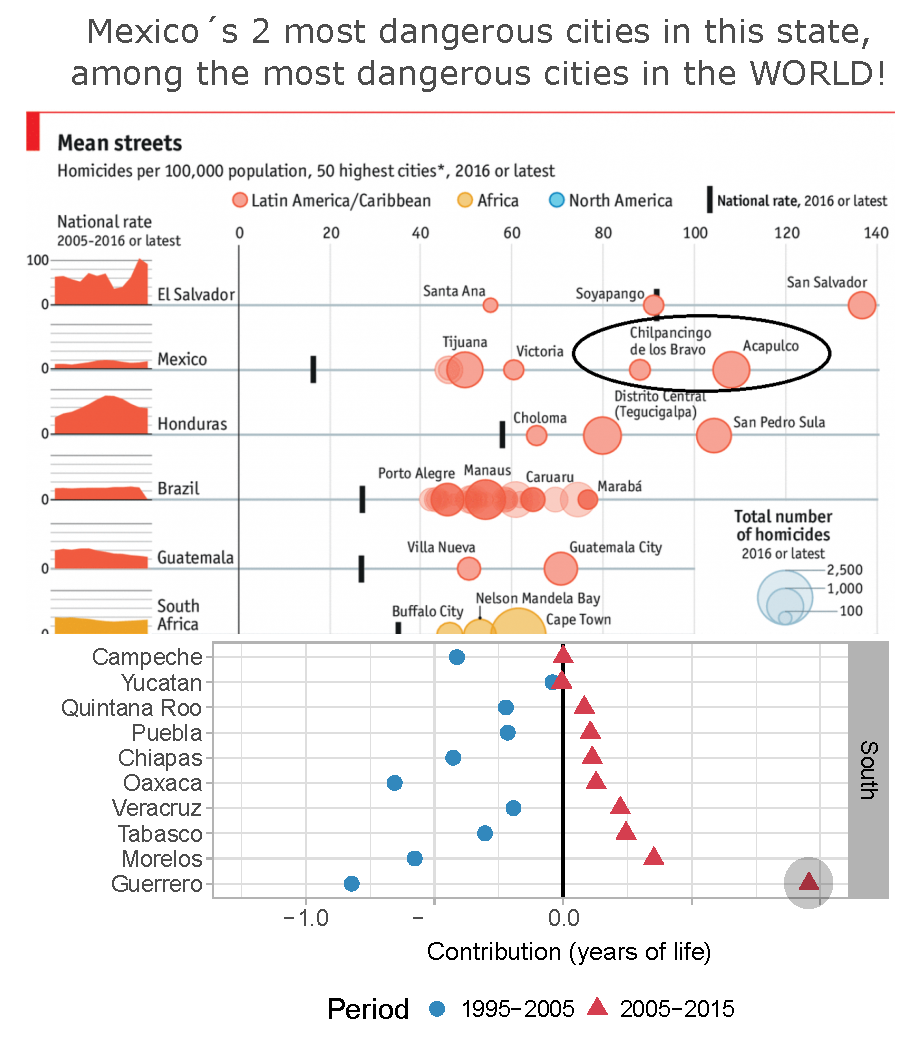
\includegraphics[scale=.47]{Figures/Figure_432}
	\end{center}
\end{frame}


\begin{frame}
\Large{
\textbf{Key messages} \pause

		\begin{itemize}
		
		\item Homicides \textbf{reversed} life expectancy gains and \textbf{increased} inequality of lifespans. \pause
		
		\item Young males \textbf{live less}, on average, and \textbf{face more uncertainty}.\pause
		
\item \textbf{Ten years into the War on Drugs}, Mexico has not been able to reduce the homicide levels to those prior to 2005 \pause
		
	    \item Failure to recognize and correct the detrimental \textbf{consequences in health and human rights} of 					violence.
							
		\end{itemize}

}
\end{frame}



\begin{frame}
\Huge{
\begin{center}
International Perspective \linebreak \\

{\fontsize{70}{80}\selectfont 

 $\backsim$ 2,000,000}\\
15-30

\end{center}
}
\end{frame}

\begin{frame}
\Huge{
\begin{center}
{\fontsize{70}{80}\selectfont 77\%}\\
Men

\end{center}
}
\end{frame}


\begin{frame}
\Huge{
\begin{center}
{\fontsize{70}{80}\selectfont 35\% Homicides}\\
(+ 1/2 million)

\end{center}
}
\end{frame}


\begin{frame}
	\begin{center}
		\large{\textbf{Life expectancy by homicide rate, males 2015.}}
 
	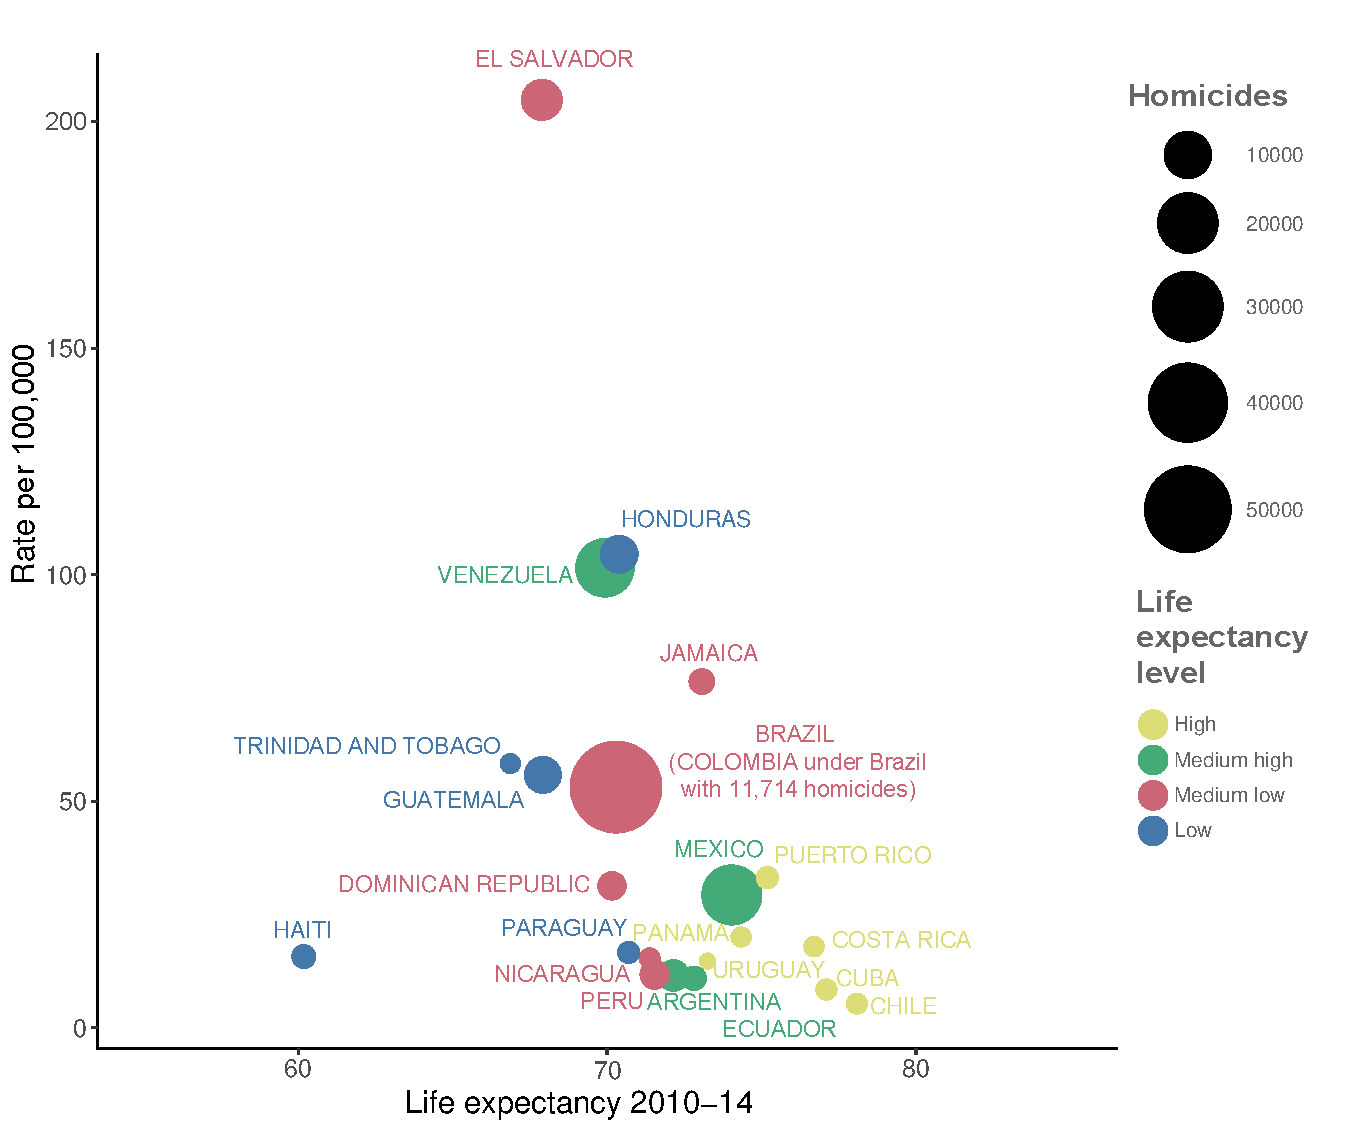
\includegraphics[scale=.42]{Figures/LACrates3}	
	
		\end{center}
	\vspace*{-.5cm}   
	\tiny{Canudas-Romo \& Aburto (forthcoming)}
\end{frame}




\begin{frame}
\Large{
\textbf{Future directions} \pause

		\begin{itemize}
		
		\item The impact of \textbf{homicides} on longevity and lifespan inequality in \textbf{Latin America.} \pause
		
		\item Is there a match between \textbf{perceived and observed vulnerability}.\pause
		
		\item How are \textbf{long-term decisions affected} by vulnerability in the context of the War on Drugs?\pause
		
		\item What is the \textbf{burden of violence} on \textbf{women}?\pause
		
		\item Violence as a \textbf{social determinant of health}.\pause
							
		\end{itemize}

}
\end{frame}



%%%%%%%%%%%%%%%%%%%%%%%%%%%%%%%%%%%%%%%%%%%%%%%%%%%%%%%%%%%%%%%%%%%%%%%%

%%%%%%%%%%%%%%%%%%%%%%%%%%%%%%%%%%%%%%%%%%%%%%%%%%%%%%%%%%%%%%%%%%%%%%%%
\begin{frame}
 \begin{center}
	\begin{center}
	 \textbf{Challenge of Mexico: Reducing violence}
	\end{center}

	\bigskip

Email: jmaburto@health.sdu.dk 

\faTwitter \quad  @jm\_aburto 

\faGithub \quad @jmaburto 

Shinnyapp: \url{<https://demographs.shinyapps.io/LVMx_15_App/>}


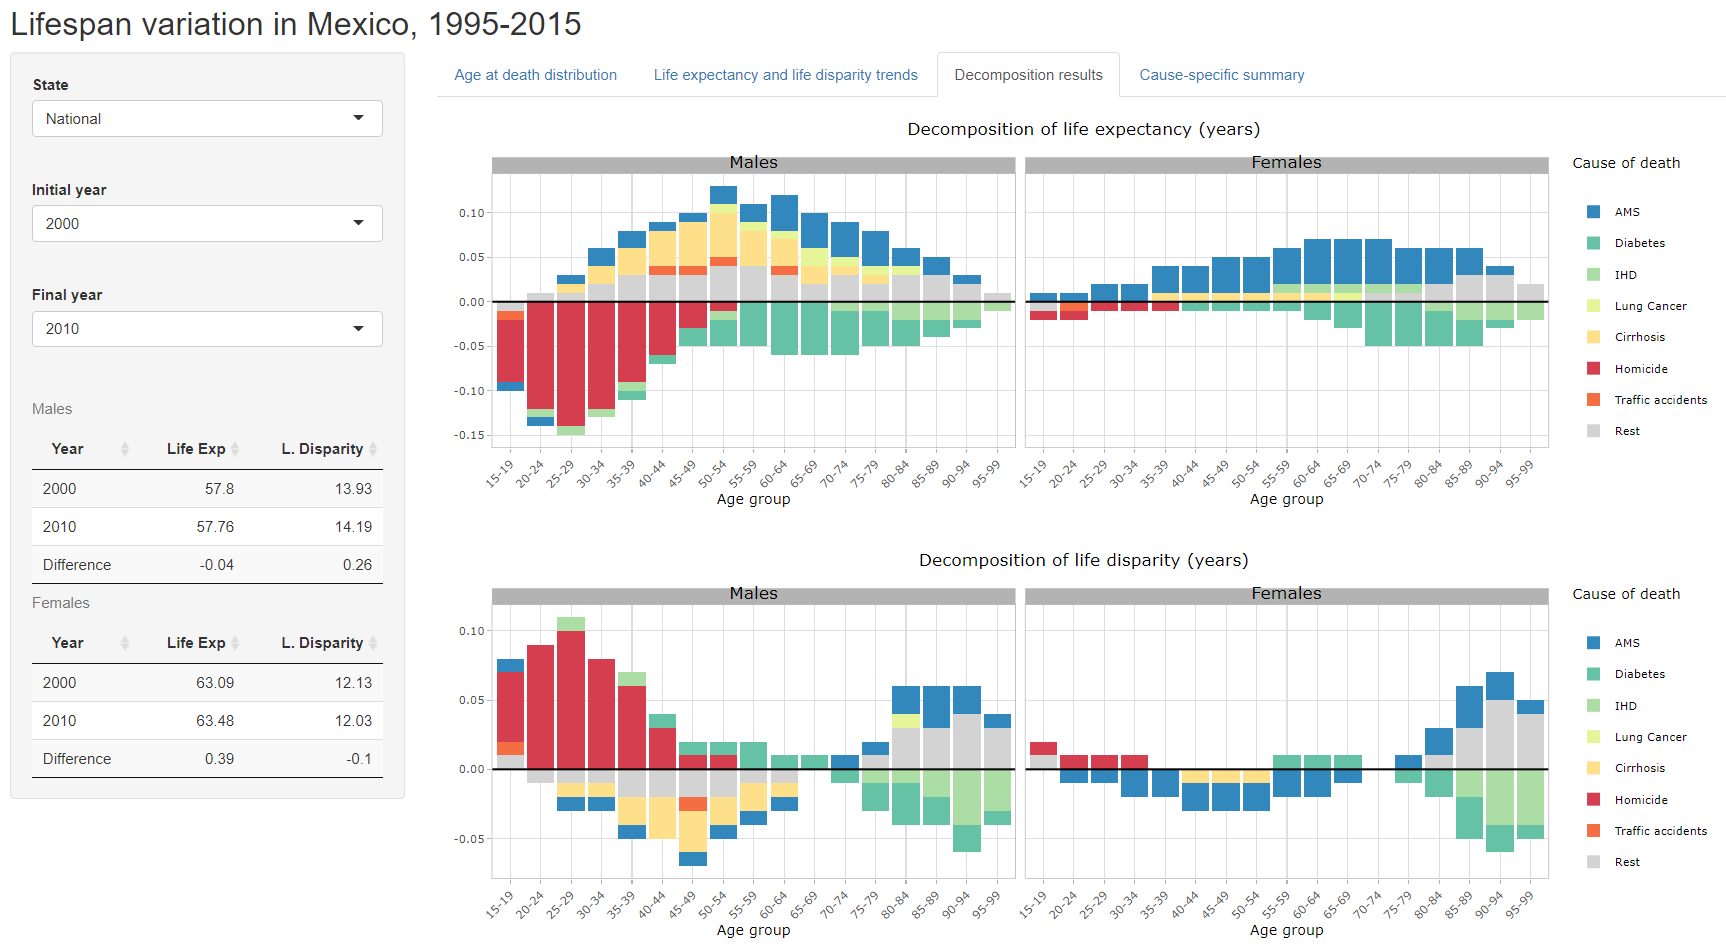
\includegraphics[scale=0.23]{Figures/Shinnyapp_fig} \\   

 

\end{center}
 
 

\end{frame}



\end{document}
	

